\documentclass{beamer}
\usetheme{CambridgeUS}
\usecolortheme{default}
\setbeamercolor{itemize item}{fg=darkred!80!black}


\makeatletter
\setbeamertemplate{footline}
{
  \leavevmode%
  \hbox{%
  \begin{beamercolorbox}[wd=.333333\paperwidth,ht=2.25ex,dp=1ex,center]{author in head/foot}%
    \usebeamerfont{author in head/foot}Candidato: F. Massa
  \end{beamercolorbox}%
  \begin{beamercolorbox}[wd=.333333\paperwidth,ht=2.25ex,dp=1ex,center]{title in head/foot}%
    \usebeamerfont{title in head/foot}Relatori: G. Chiarelli, C. Gemme
  \end{beamercolorbox}%
  \begin{beamercolorbox}[wd=.333333\paperwidth,ht=2.25ex,dp=1ex,right]{date in head/foot}%
    \usebeamerfont{date in head/foot}23 Settembre 2016\hspace*{2em}
    \insertframenumber{} / \ref{Conclusions}\hspace*{2ex} 
  \end{beamercolorbox}}%
  \vskip0pt%
}
\makeatother

\setbeamercolor{section in head/foot}{fg=white, bg=darkred!95!white}

\setbeamercolor{palette quaternary}{use=structure, bg=darkred!80!black} % changed this


\setbeamertemplate{headline}{%
\leavevmode%
  \hbox{%
    \begin{beamercolorbox}[wd=\paperwidth,ht=2.5ex,dp=1.125ex]{palette quaternary}%
    \insertsectionnavigationhorizontal{\paperwidth}{}{\hfill \hfill}
    \end{beamercolorbox}%
  }
}

\title{Tracking Performances of the ATLAS detector \\
for the HL-LHC in the 
$H \rightarrow ZZ^{*} \rightarrow 4\mu$ channel}
%\subtitle{Laurea Magistrale in Fisica}
%\author{Federico Massa}
\institute{\large{Laurea Magistrale in Fisica \\
Universit\`a di Pisa}}
\date{\small 23 Settembre 2016}

%\setbeameroption{show notes}
\setbeameroption{hide notes}
\setbeamertemplate{navigation symbols}{}

\usepackage{tikz}
\usetikzlibrary{decorations.pathreplacing}
\usetikzlibrary{positioning, calc}
\newcommand{\tikzmark}[1]{\tikz[overlay,remember picture] \node (#1) {};}

\usepackage{amsmath}% mathtools includes this so this is optional
\usepackage{mathtools}
\usepackage[export]{adjustbox}
\usepackage{tcolorbox}
\definecolor{dred}{RGB}{200, 0, 0}

\begin{document}

%-----------------------------------------

{\setbeamertemplate{footline}{}
\setbeamertemplate{headline}{}
\begin{frame}
\titlepage
\begin{columns}[t]
\begin{column}{.1\textwidth}
\end{column}
\begin{column}{.65\textwidth}
\textbf{Relatori:}\\[0.05cm]
Giorgio Chiarelli \\
Claudia Gemme
\end{column}
\begin{column}{.25\textwidth}
\textbf{Candidato:}\\[0.05cm]
Federico Massa
\end{column}

\end{columns}
\end{frame}}
\addtocounter{framenumber}{-1}

\begin{frame}
\setbeamercolor{normal text}{fg=dred,bg=}
%\setbeamercolor{alerted text}{fg=dred,bg=}
\usebeamercolor{normal text}

\setbeamercovered{dynamic}

\frametitle{Struttura della presentazione}
\setbeamercolor{local structure}{fg=dred}
\begin{itemize}[<+->]
\item LHC e l'esperimento ATLAS
\vskip0.5cm
\item {Fase di alta luminosit\`a di LHC}
\vskip0.5cm
\item {Upgrade del rivelatore interno}
\vskip0.5cm
\item {Tecnica di simulazione veloce}
\vskip0.5cm
\item {Studio di singola particella}
\vskip0.5cm
\item {Misura del canale $H\rightarrow 4\mu$}
\vskip0.5cm
\end{itemize}

\end{frame}

\section{Introduzione}

\begin{frame}[t]
\frametitle{Il Large Hadron Collider (LHC)}
\centering
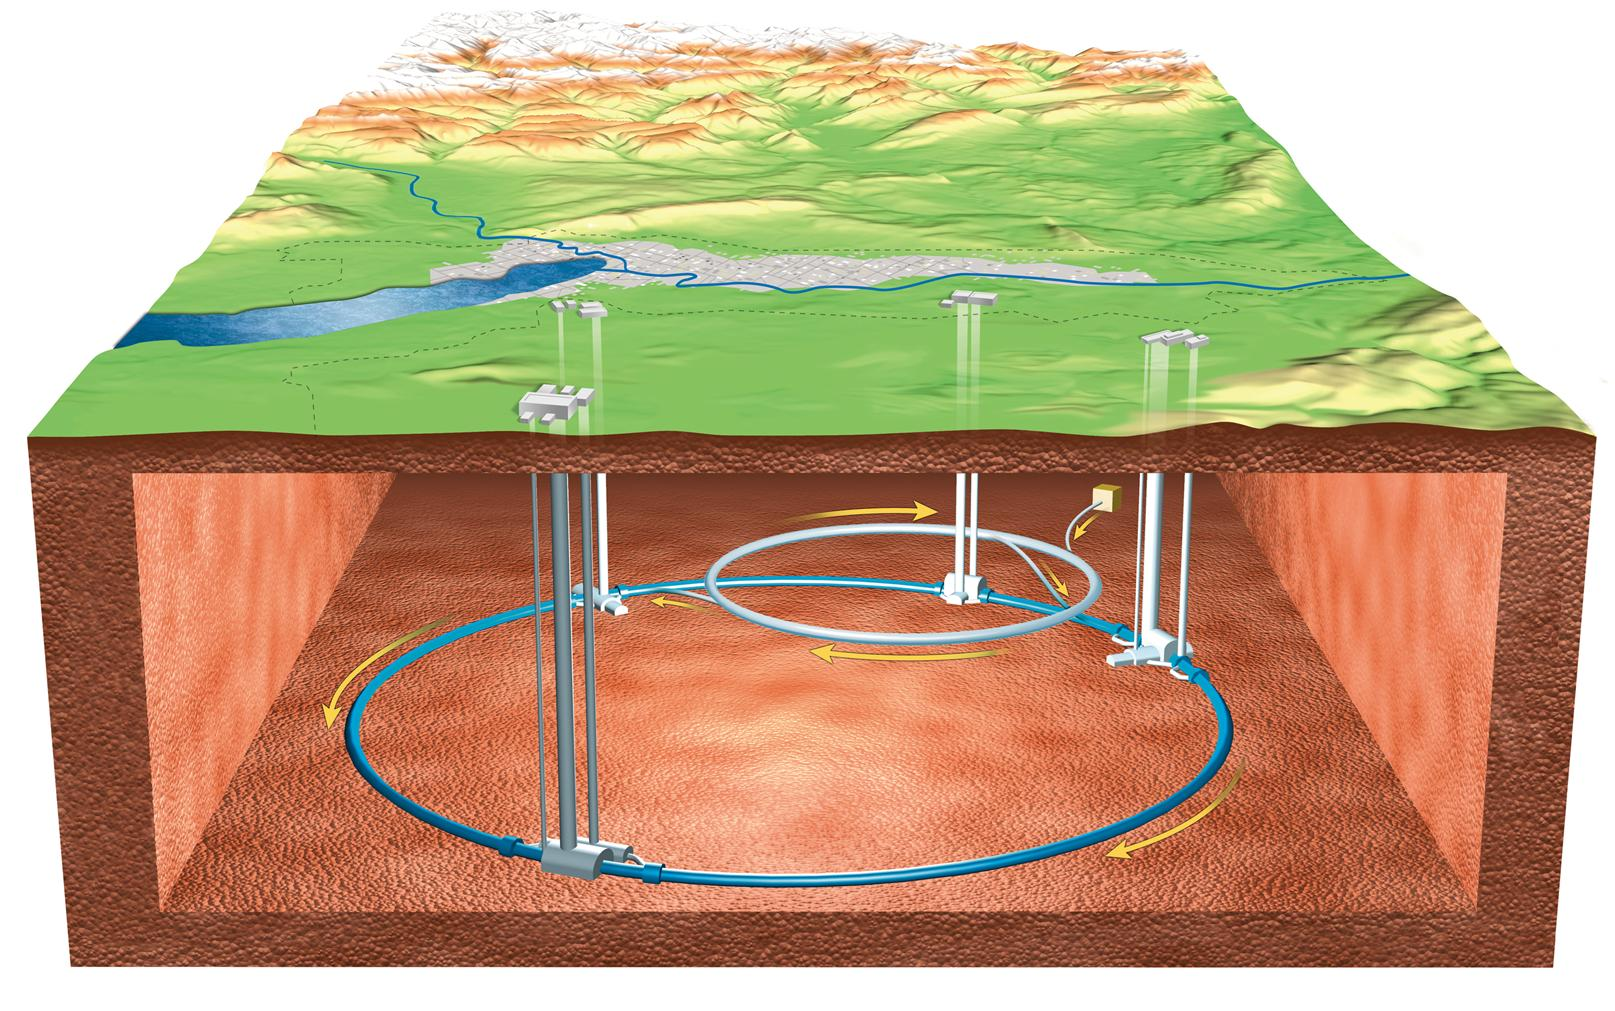
\includegraphics[width=.7\textwidth]{lhc-subterraneo}

\note<1>{
Qui dico che LHC è un sincrotrone che accelera protoni e li fa scontrare
in corrispondenza dei 4 esperimenti, tra i quali ATLAS che è quello di cui
ci siamo occupati. Poi compare l'itemize in cui dico che attualmente sono ad un'energia
di 13 TeV e che ci sono tot bunch ogni 25 ns
}

\onslide<2->{
\begin{itemize}
\item Durante la presa dati attuale (Run 2), i protoni collidono ad un'energia del centro di massa di 13 TeV
\item $\sim$ 2800 ``pacchetti'' (\textit{bunch}) di protoni collidono ogni 25 ns
\end{itemize}}

\end{frame}

%-----------------------------------------

\begin{frame}[t]
\frametitle{Tipi di collisione}
\note<1>{
Abbiamo visto che LHC accelera protoni e fa scontrare i bunch. Cosa succede in una singola
collisione? Pu\`o esserci collisione elastica, pu\`o esserci una collisione inelastica in cui si 
osservano un gran numero di prodotti finali, e ci sono
i processi hard, in cui i quark interagiscono direttamente per dare luogo a interazioni rare ``interessanti''.
}
Le collisioni possono essere:
\begin{itemize}
\item \textbf{elastiche}: i protoni rimangono intatti
\item \textbf{anelastiche}: lo stato finale è diverso da quello iniziale
	\setbeamercolor{local structure}{fg=red}
	\begin{itemize}
	\item \textbf{di ``hard-scattering''}: la collisione avviene direttamente tra partoni con produzione di uno stato finale raro
	\end{itemize}
\end{itemize}

\centering
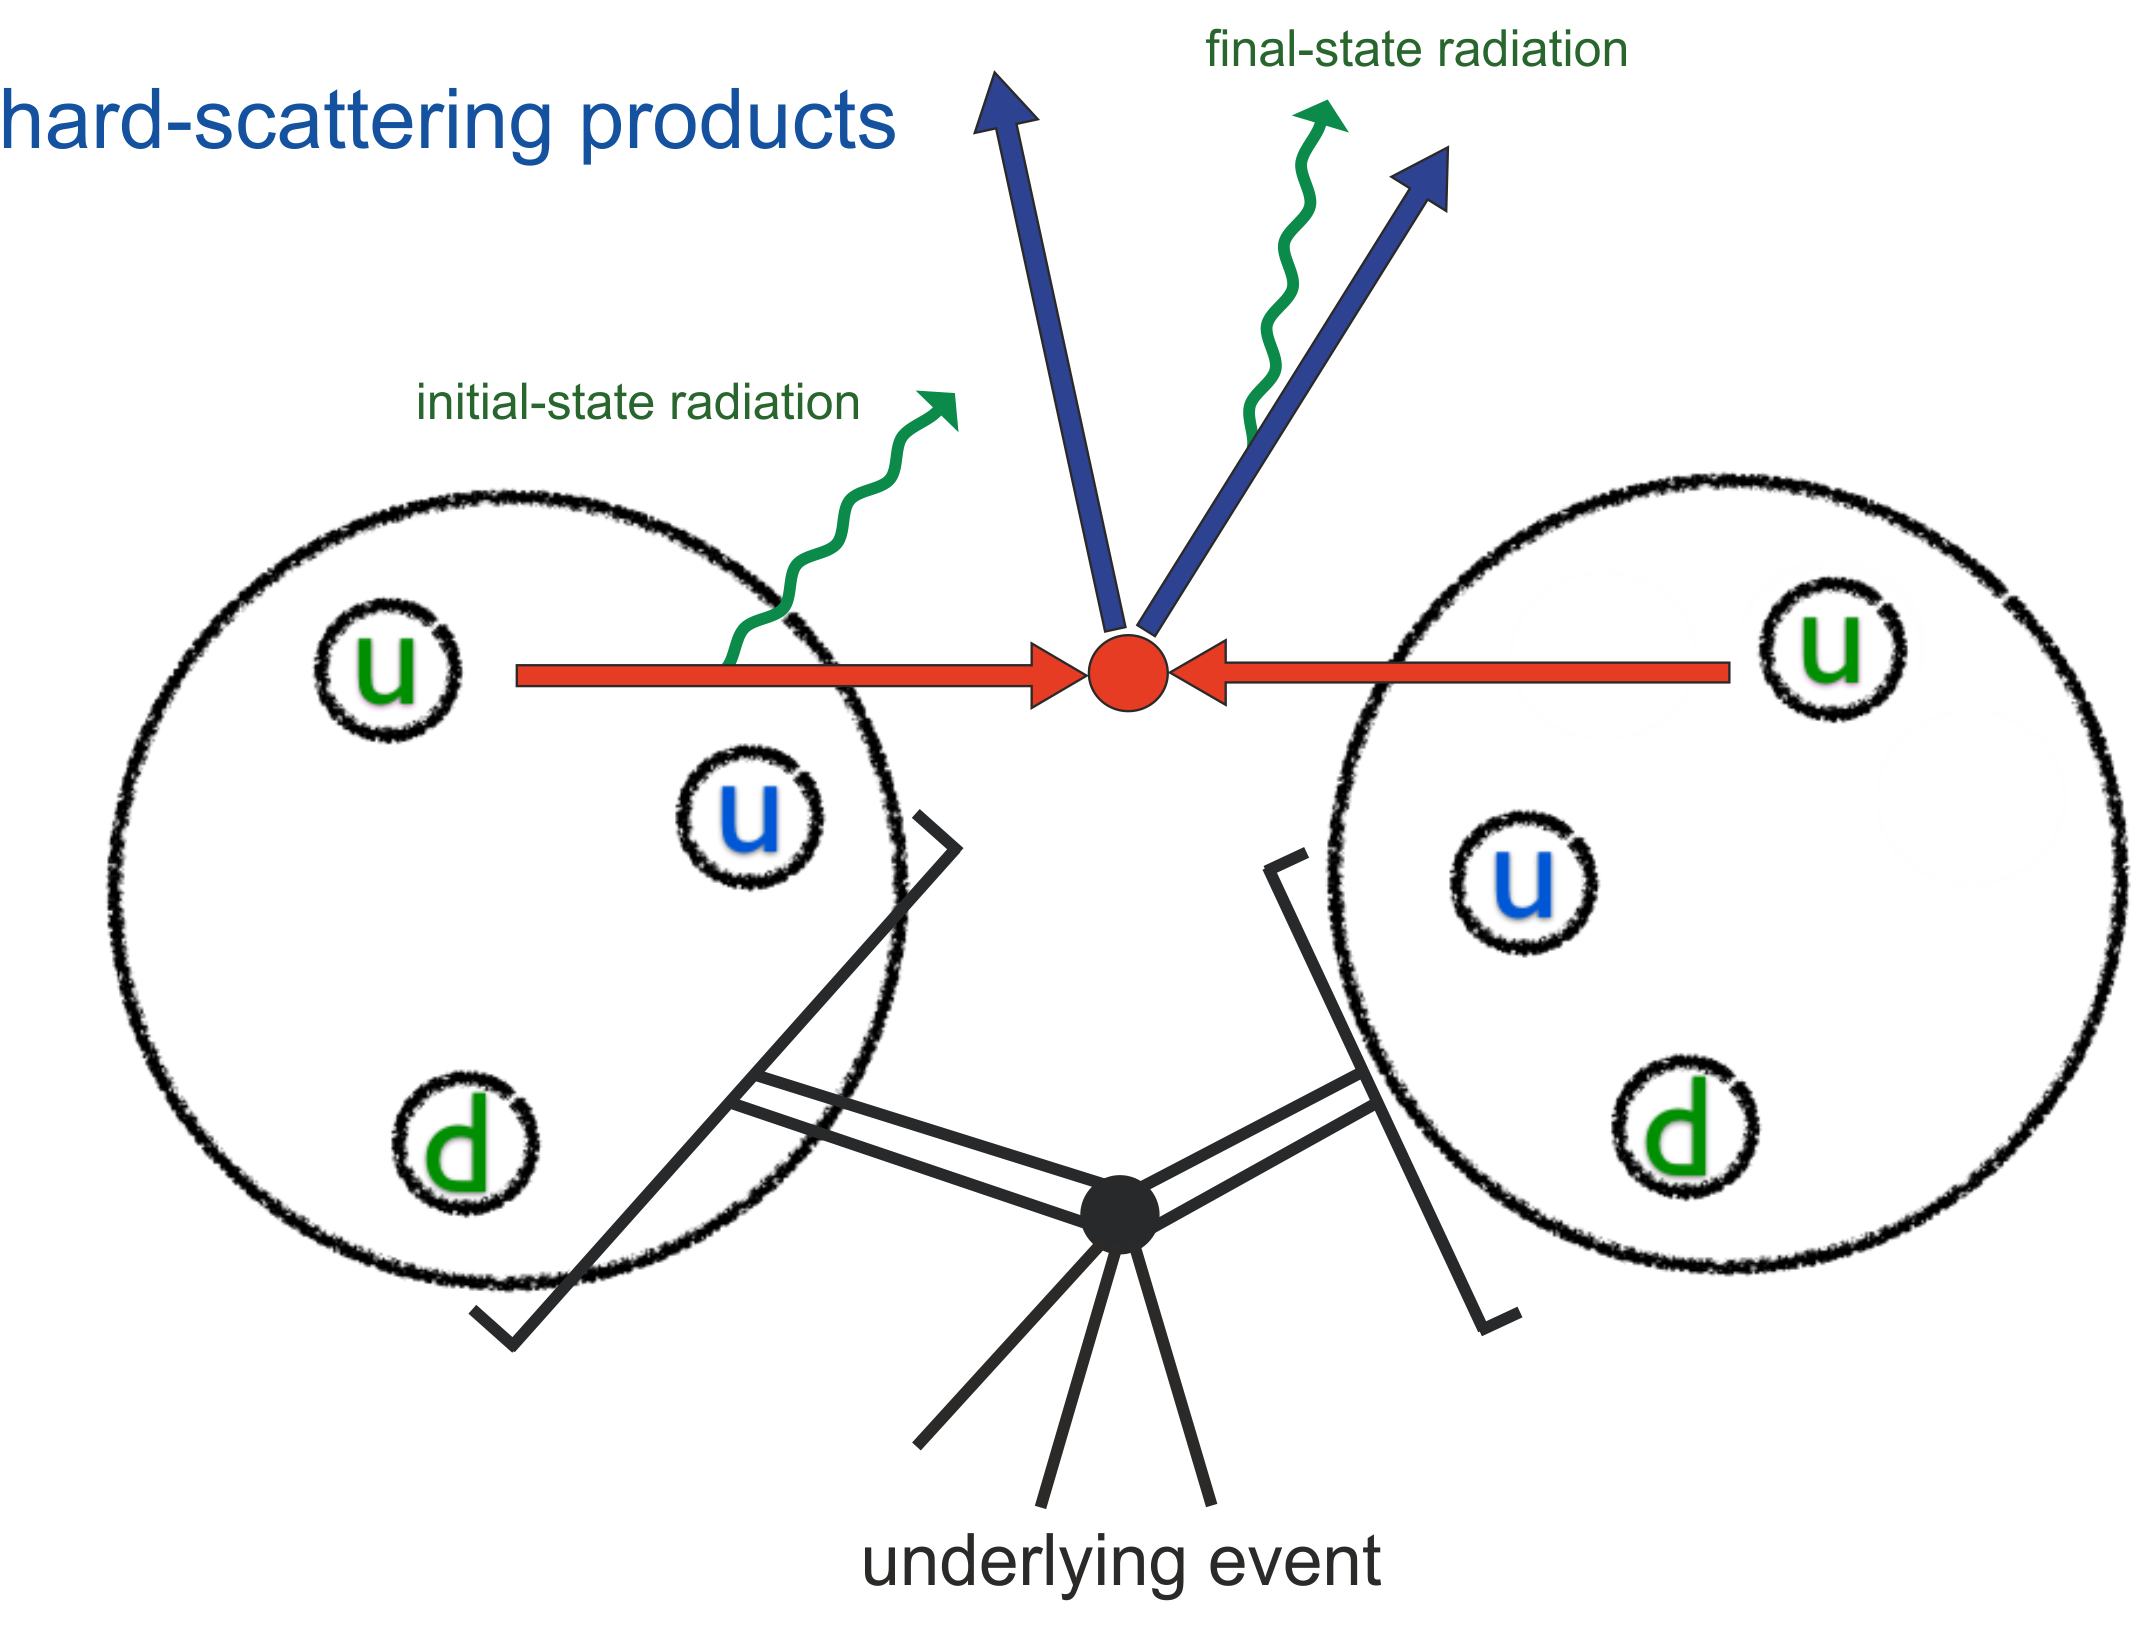
\includegraphics[width=.5\textwidth]{collision1}


\end{frame}

%-----------------------------------------

\begin{frame}[t]
\frametitle{Numero di interazioni}

\note<1>{
Definisco R = L$\sigma$  e dico che il numero di interazioni per bunch è dato da N = L$\times \sigma_{inel.} \times 25$ ns
}

Il numero medio di interazioni per unit\`a di tempo \`e dato da\\
\medskip

\begin{columns}
\begin{column}{0.4\textwidth}
$$
\frac{dN}{dt} =\sigma \times \mathcal{L}
$$
\end{column}
\begin{column}{0.6\textwidth}
\end{column}
\end{columns}
\medskip
con:\\
\begin{itemize}
\item $\sigma$: \textbf{sezione d'urto} del processo considerato
\item $\mathcal{L}$: \textbf{luminosit\`a istantanea}, numero di collisioni 
per unit\`a di tempo e di area
\item $\int\mathcal{L}dt$: \textbf{luminosit\`a integrata} nel tempo di presa dati
\end{itemize}
\bigskip 

\onslide<2->{
Il numero medio di interazioni per ``bunch-crossing'' \`e quindi:\\
\begin{columns}
\begin{column}{0.6\textwidth}
$$
\langle\mu\rangle \propto \sigma_{inel.} \times \mathcal{L} \mathrm{\mathbf{\ \simeq 23\ }(Run 2)} 
$$
\end{column}
\begin{column}{0.4\textwidth}
\end{column}
\end{columns}

}
\end{frame}

%-----------------------------------------

\begin{frame}

\frametitle{Il rivelatore di ATLAS}
\begin{columns}
\begin{column}{0.6\textwidth}
\centering
\includegraphics<1>[width=\textwidth]{atlas}
\includegraphics<2>[width=\textwidth]{atlas_2}
\end{column}
\begin{column}{0.4\textwidth}
	\begin{itemize}
	\item {\small \textbf{Solenoide e toroidi:} producono un campo magnetico che fa curvare
	le particelle cariche}
	\item {\small \textbf{Rivelatore interno:} ricostruisce i vertici e le tracce delle particelle cariche, in particolare misurandone l'impulso}
	\item {\small \textbf{Calorimetri:} misurano l'energia di particelle cariche e neutre}
	\item {\small \textbf{Camere dei muoni:} misurano le tracce dei muoni}
	\end{itemize}
\end{column}
\end{columns}
\end{frame}

%-----------------------------------------

\begin{frame}
\frametitle{Il Rivelatore Interno}
\centering

\begin{center}
        \begin{tikzpicture}
            \node[anchor=south west,inner sep=0] (image) at (0,0) {\includegraphics[width=.85\textwidth]{NewID}};
            \node[align=center,red] at ($(image.south east) + (2,1.4)$) {\vbox{\small
            \begin{itemize}
		\item $\eta = -\log{(\tan{\frac{\theta}{2}})}$
		\item Copertura angolare: $|\eta| < 2.5$
		\item 4 strati di Pixel
		\item 4 strati di microstrip (SCT) 
		\item Transition Radiation Tracker (TRT)
            \end{itemize}}};
        \end{tikzpicture}
    \end{center}

\end{frame}

%-----------------------------------------
\begin{frame}
\frametitle{High Luminosity LHC (HL-LHC)}
\onslide<1-> {
LHC prevede una serie di upgrade per aumentare la luminosit\`a istantanea \\
\ \ \ \ \ \ \ \ \ \ \  $\rightarrow$ \textbf{High-Luminosity LHC} (HL-LHC)

Aumento del numero di interazioni per unit\`a di tempo (N $\propto \sigma \times \mathcal{L}$):\\
\begin{itemize}
\item Possibilit\`a di osservare canali pi\`u rari
\item Miglioramento delle misure sugli accoppiamenti e le sezioni d'urto
\item Miglioramento dei limiti o scoperta di nuova fisica
\end{itemize}}

\onslide<2->{
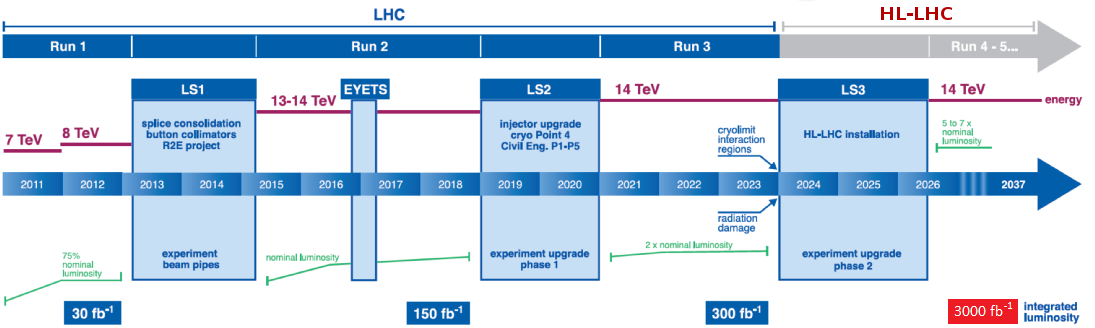
\includegraphics[width=\textwidth]{HLLHC_Plan_2}}

\end{frame}

%-----------------------------------------
\begin{comment}
\begin{frame}[t]
\frametitle{High Luminosity LHC (HL-LHC) - 2}
\note<1>{
Sono previsti una serie di upgrade ad LHC, in particolare quello del 2026 che porterà ad HL-LHC, in cui la luminosit\`a 
passer\`a dal valore attuale di $10^{34}$ a 7.5 x $10^{34}$ e prevede di durare 10 anni, raccogliendo 3000 fb$^{-1}$ di dati a 14 TeV.
}


\vskip0.2cm
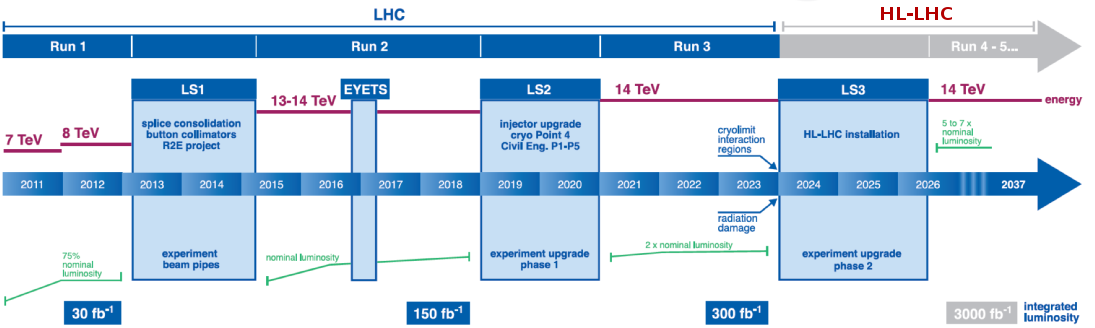
\includegraphics[width=\textwidth]{HLLHC_Plan}

\begin{columns}
\begin{column}{0.7\textwidth}
\end{column}
\begin{column}{0.3\textwidth}

\begin{tikzpicture}[scale=1]
\draw [decorate,decoration={brace,amplitude=8pt},xshift=-50pt,yshift=0pt, dred, thick]
(3.5,0) -- (0,0); %node [midway,xshift=-0cm]{};
\end{tikzpicture}
\end{column}
\end{columns}
\medskip
\begin{itemize}
\item HL-LHC prevede di raccogliere una luminosit\f`a integrata di 3000 fb$^{-1}$
\item Massima luminosit\`a istantanea: 7.5 $\times 10^{34}$ cm$^{-2}$s$^{-1}$
\item L'energia del centro di massa sar\`a quella di progetto: 14 TeV
\end{itemize}

\end{frame}
\end{comment}
%-----------------------------------------

\begin{frame}[t]
\frametitle{Pile-up}
Il numero di collisioni per ``bunch-crossing'' ad HL-LHC aumenta
a causa dell'aumento della luminosit\`a e della sezione d'urto inelastica 
($\langle\mu\rangle \propto \sigma_{inel} \times \mathcal{L}$)\\

\begin{itemize}
\item Le collisioni che avvengono \textit{nello stesso bunch} di quella di interesse
rappresentano il cosiddetto \textbf{in-time pile-up}, mediamente $\langle\mu\rangle$
\item valore nominale ad HL-LHC: 140
\item valore di picco ad HL-LHC: 200
\end{itemize}

\only<1>{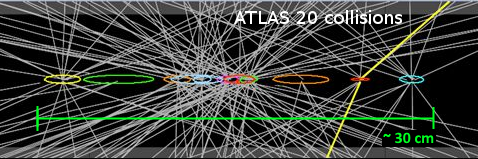
\includegraphics[width=\textwidth]{collisions20_2}}
\only<2>{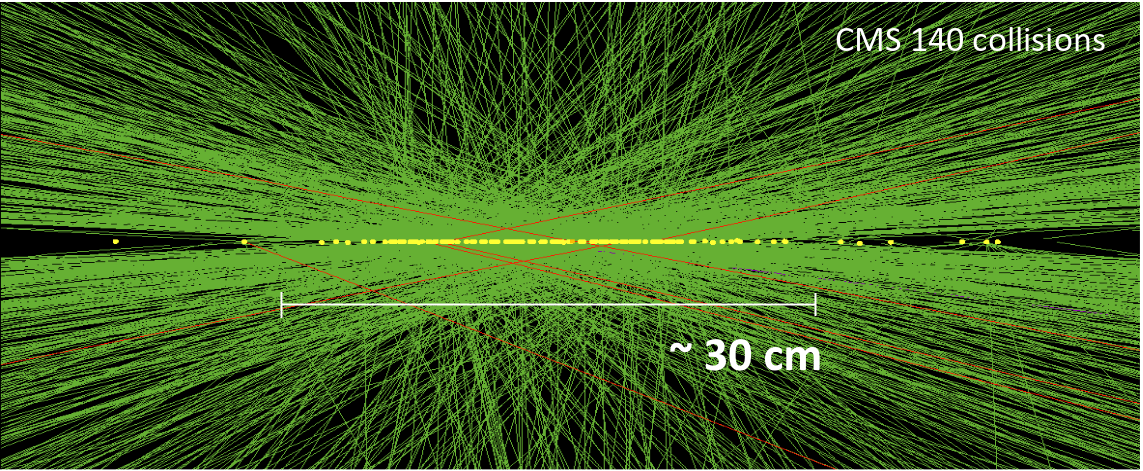
\includegraphics[width=\textwidth, height=4cm]{collisions140_2}}



\end{frame}

%-----------------------------------------

\begin{frame}
\frametitle{Upgrade del rivelatore interno}
L'attuale rivelatore interno \`e inadatto alla fase di alta luminosit\`a:
\pause
\begin{itemize}
\item<+-> I rivelatori a pixel e SCT non sono disegnati per sopportare l'alto
flusso di radiazione di HL-LHC
\item<+-> L'elettronica di read-out \`e disegnata per un numero massimo di eventi
		di pile-up di 50 $\rightarrow$ inefficienze ad HL-LHC
\item<+-> La risoluzione spaziale dell'SCT non permette di risolvere tracce
		in ambienti altamente densi di particelle
\item<+-> Il TRT raggiunger\`a il 100\% di occupancy (frazione di canali elettronici attivi)
\end{itemize}

\bigskip

\onslide<+->{\Large{\color{dred}\textbf{\ \ \ $\rightarrow$ Necessario upgrade: Inner Tracker (ITk)}}}

\end{frame}

%-----------------------------------------
\begin{comment}
\begin{frame}
\frametitle{Layout di ITk: Step-1}


\begin{columns}
\begin{column}{0.5\textwidth}
	\begin{itemize}
	\small
	\item Copertura angolare estesa: $|\eta| < 2.5 \rightarrow 4.0$
	\item 5 strati di pixel + 4 SCT (no TRT)
	\item Pixel a maggiore risoluzione
	\item Strip pi\`u corte
	\end{itemize}
	\ \ \ \
\end{column}
\begin{column}{0.5\textwidth}
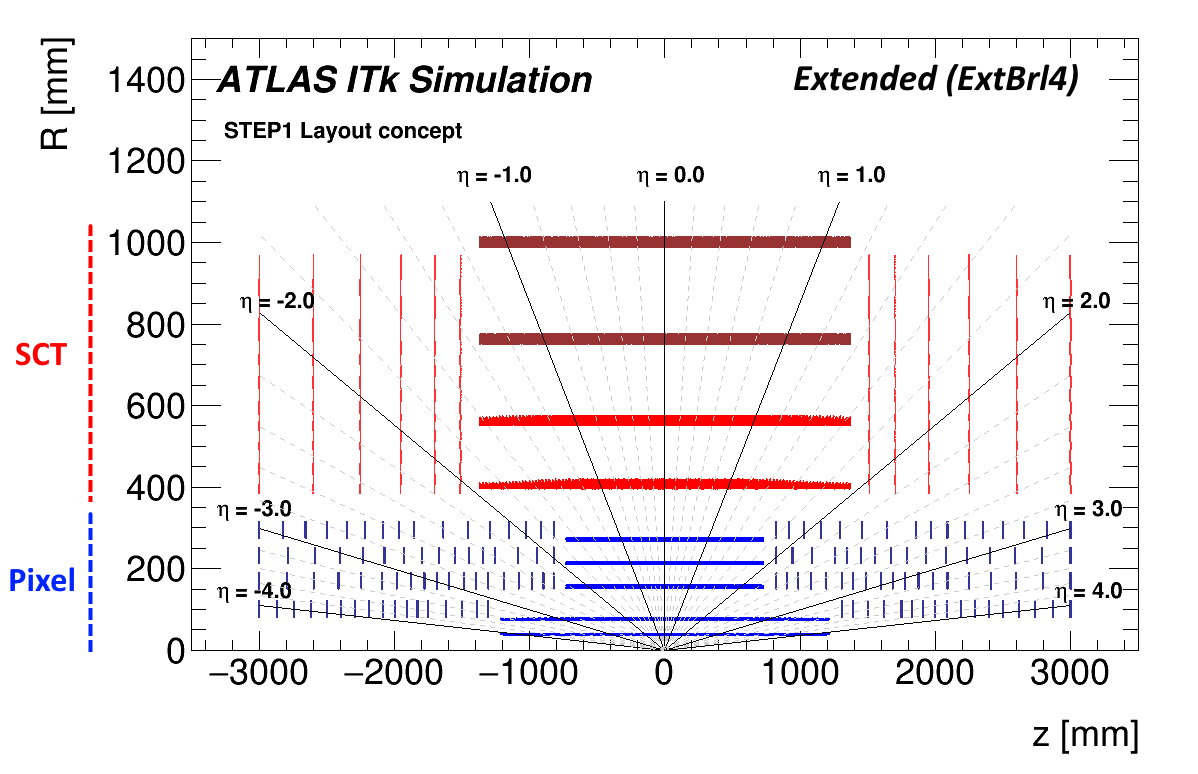
\includegraphics[width=\textwidth,height=3.8cm]{ExtBrl4_2}
\end{column}
\end{columns}

\begin{columns}
\begin{column}{0.5\textwidth}
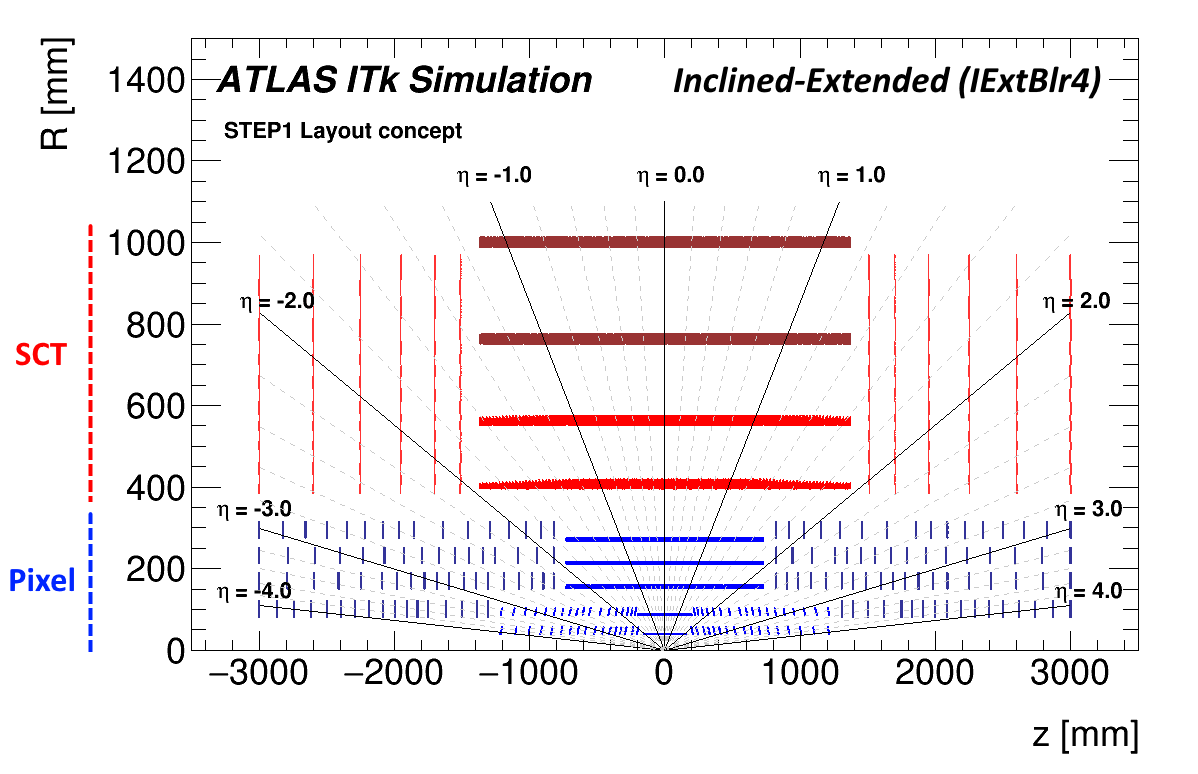
\includegraphics[width=\textwidth,height=3.8cm]{IExtBrl4_2}
\end{column}
\begin{column}{0.5\textwidth}
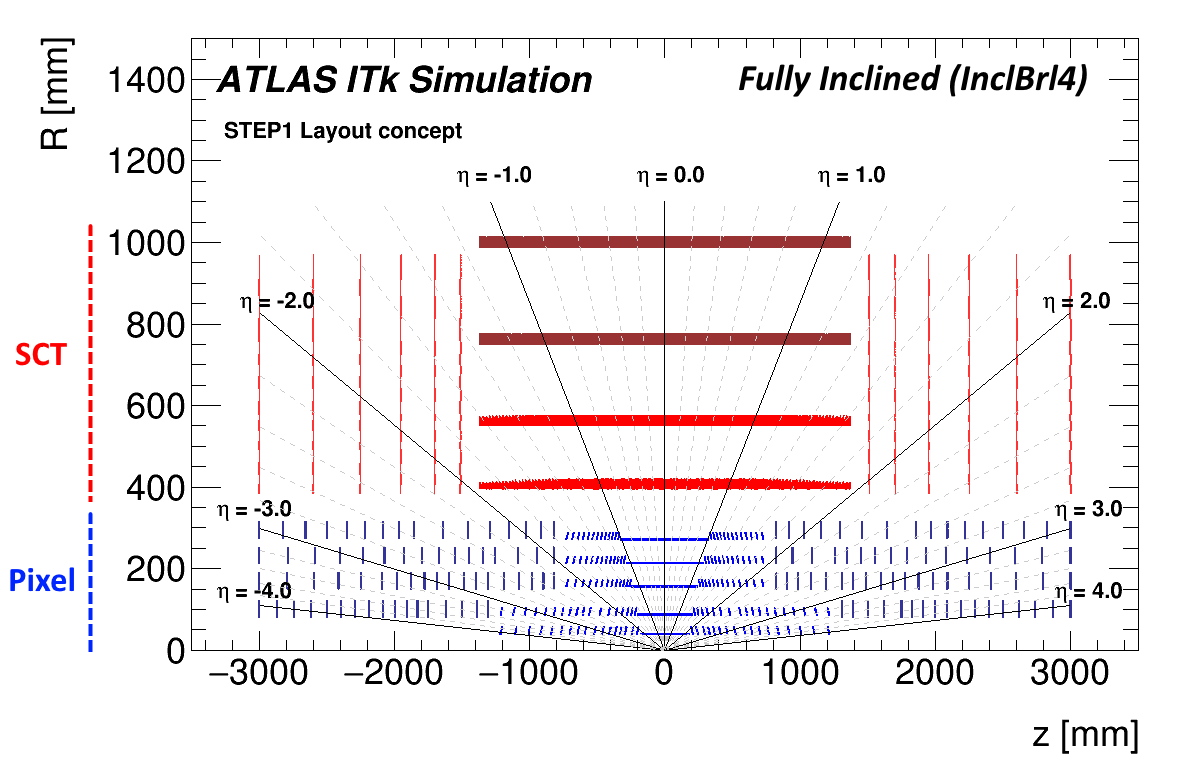
\includegraphics[width=\textwidth,height=3.8cm]{InclBrl4_2}
\end{column}
\end{columns}

\end{frame}
\end{comment}
%-----------------------------------------
\begin{frame}
\frametitle{Layout di ITk: Step-1}
\includegraphics<1>[width=\textwidth]{ExtBrl4_2}
\includegraphics<2>[width=\textwidth]{IExtBrl4_2}
\includegraphics<3>[width=\textwidth]{InclBrl4_2}
\end{frame}
%-----------------------------------------
\begin{frame}[t]
\frametitle{Inclined sensors}
\begin{center}
InclBrl4: Pixel Layout
\begin{tikzpicture}

\onslide<1->{
    \node[anchor=south west,inner sep=0] (fig) at (0,0) {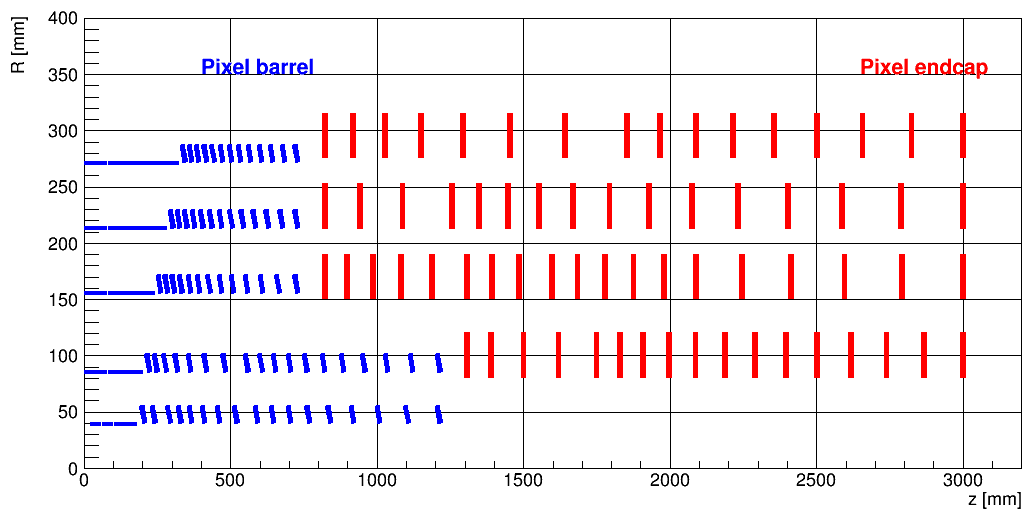
\includegraphics[width=.8\textwidth]{InDetPixelLayoutRZ}};
    }
\onslide<2->{
    \path let       \p1 = ($(fig.north west)$),
			\p2 = ($(fig.south east)$),
			\n{figheight} = {veclen(\y1,\y2)},
			\n{figwidth} = {veclen(\x1,\x2)},
			\p3 = ($(\p1) - (0,\n{figheight}) + (.22*\n{figwidth},.25*\n{figheight})$)  in
	node (rect) at (\p3) [draw,black,thick,minimum width=.05*\n{figwidth},minimum height=.18*\n{figheight}] {};
	%\draw<2->[red] (2.45,1) rectangle (3,2);    
    \node[anchor=south west,inner sep=0] (zoom) at (4,-1.9) {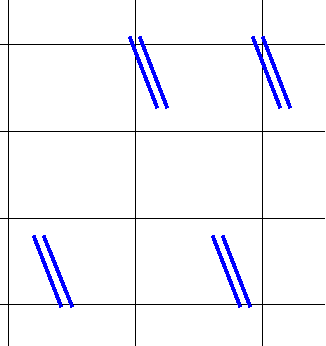
\includegraphics[cfbox=black 4pt,width=.2\textwidth]{InclZoom}};

\path let \p4 = ($(zoom.south east)$),
		\p5 = ($(fig.south east)$),
		\p6 = ($(zoom.south west)$),
		\p7 = ($(zoom.north west)$),
		\n{zoomheight} = {veclen(\y6, \y7)}
			in
		
coordinate (zoomEdge) at (\x6, \y6 + \n{zoomheight}*0.75);
%coordinate (zoomEdge) at (\x6, \y6);

    \draw [black,thick] (rect.south east) -- ($(zoomEdge)$);
    %\draw [black,thick] (rect.south west) -- ($(zoom.south west)$);
    %\draw [black,thick] (rect.north west) -- ($(zoom.north west)$);
    %\draw [black,thick] (rect.north east) -- ($(zoom.north east)$);
    }
\end{tikzpicture}
\end{center}

\end{frame}

\section{Simulazione}
%-----------------------------------------
\begin{frame}
\frametitle{Simulazione standard di ATLAS}
\begin{onlyenv}<1-10>
\includegraphics<1>[width=0.9\textwidth]{SimulationFlow8}
\includegraphics<2>[width=0.9\textwidth]{SimulationFlow7}
\includegraphics<3>[width=0.9\textwidth]{SimulationFlow6}
\includegraphics<4>[width=0.9\textwidth]{SimulationFlow5}
\includegraphics<5>[width=0.9\textwidth]{SimulationFlow4}
\includegraphics<6>[width=0.9\textwidth]{SimulationFlow3}
\includegraphics<7>[width=0.9\textwidth]{SimulationFlow2}
\includegraphics<8->[width=0.9\textwidth]{SimulationFlow}
\pause
\pause
\pause
\pause
\pause
\pause
\pause
\pause
\begin{tcolorbox}{}
\onslide<+->{\small \textbf{Problema:} la simulazione del rivelatore interno ad HL-LHC impiega \\
 $\sim$ \textbf{1 ora/evento}} 
\onslide<+->{\textbf{\color{dred} $\rightarrow$ Tecniche di simulazione veloce}}
\end{tcolorbox}
\end{onlyenv}

\end{frame}

%-----------------------------------------
\begin{frame}[t]
\frametitle{Simulazione veloce del rivelatore interno}

\begin{columns}
	\begin{column}{.45\textwidth}
	\begin{tcolorbox}{}
	\textbf{\color{dred} Idee chiave:}\\
	\begin{itemize}
	\item[\color{black}-]
	 \small Simulare solo le \\ 
	 \mbox{particelle all'interno di} \mbox{regioni di interesse (\textit{RoI})}
	 attorno alle particelle di ``hard-scattering''
	 \item[\color{black}-] Simulare solo rivelatore interno
	 \end{itemize}
	\end{tcolorbox}		
	
	\end{column}
	\begin{column}{.55\textwidth}
		\centering
	%	\vskip-1.4cm
		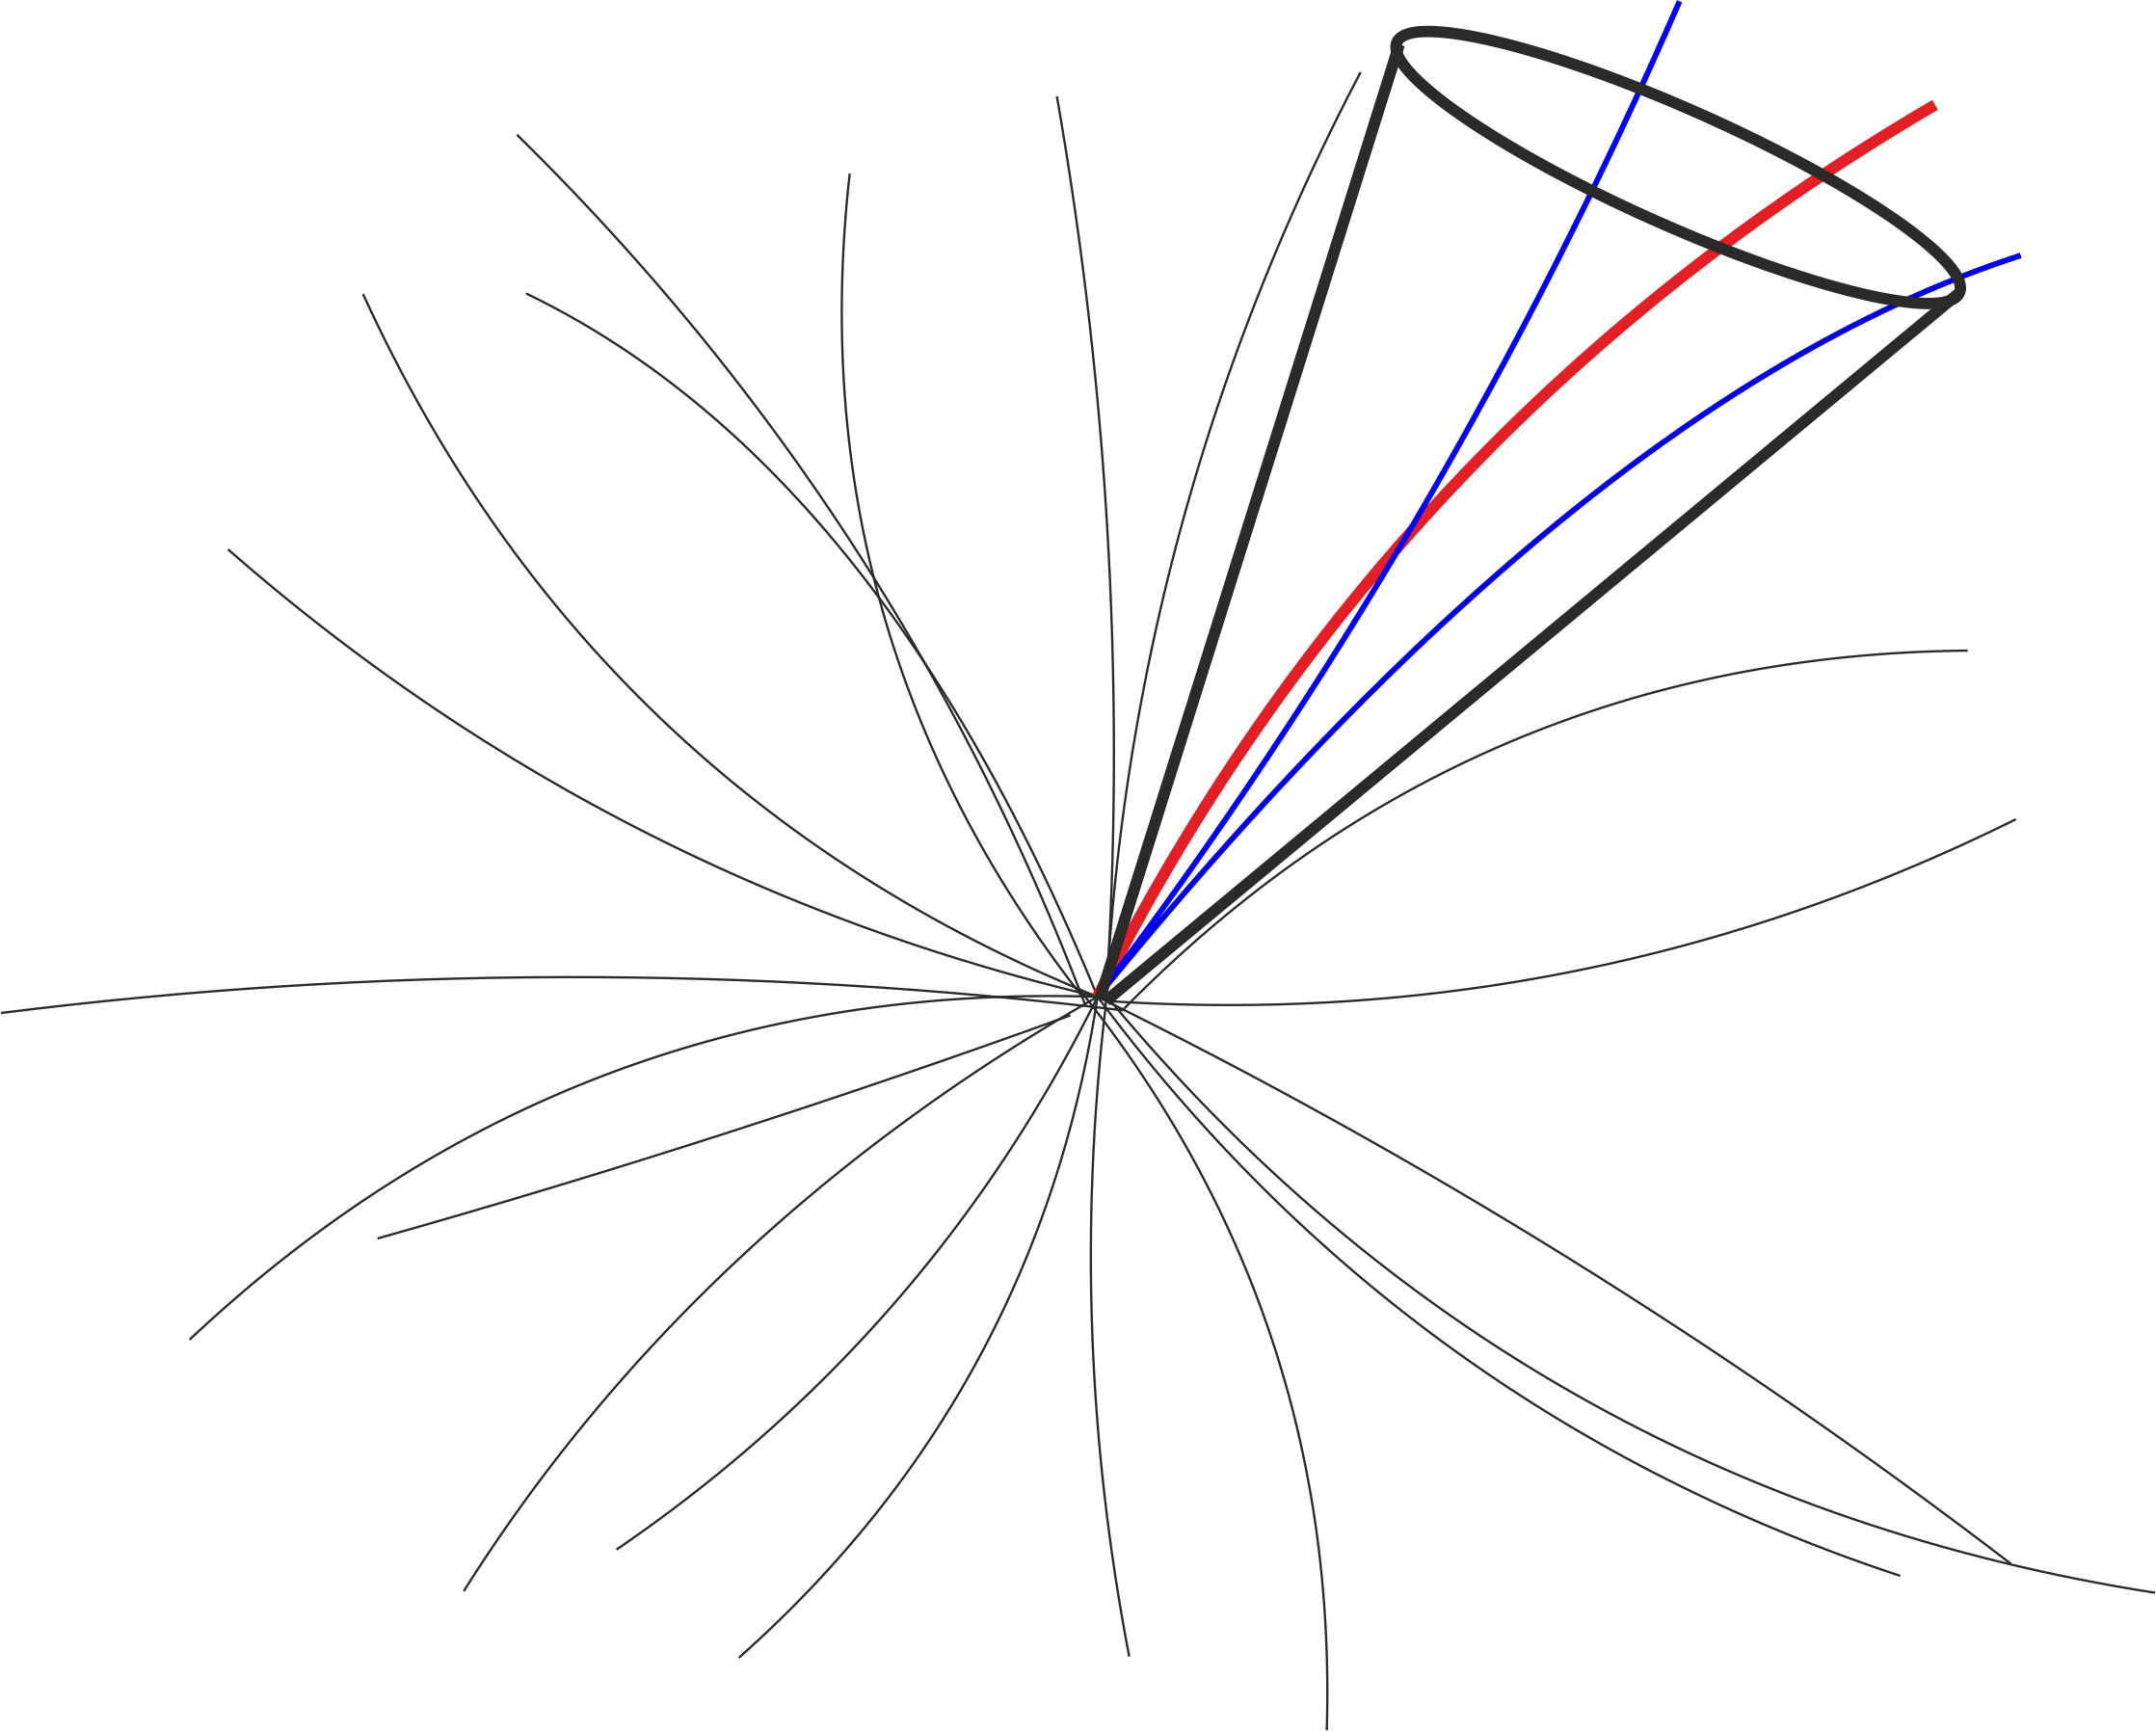
\includegraphics[width=.8\textwidth]{cone}
	\end{column}
\end{columns}

\begin{columns}
\begin{column}{.45\textwidth}
		\begin{block}{}
		Ampiezza del cono:\\
		$\Delta$R = $\sqrt{\Delta\eta^{2} + \Delta\phi^{2}}$ = 0.1
		\end{block}
\end{column}
\begin{column}{.55\textwidth}
		\begin{center}
		\small
		{\color{dred} Particella di ``hard-scattering''} \\
		\vskip0.2cm
		{\color{blue} Particelle di pile-up in RoI} \\
		\vskip0.2cm
		{\color{gray} Particelle di pile-up escluse} \\
		\vskip0.2cm
		\end{center}
\end{column}
\end{columns}
	
\end{frame}

\section{}
%-----------------------------------------
\begin{frame}


\Large{\color{dred}1. Studio di singola particella}\\
\bigskip
\bigskip
\bigskip
\Large{\color{gray}2. Studio del canale $H \rightarrow ZZ^{*} \rightarrow 4\mu$}

\end{frame}
\section{Studio di singolo $\pi^{\pm}$}
%-----------------------------------------

\begin{frame}
\frametitle{Motivazioni dello studio}

In questo studio:\\
\textbf{singolo \boldmath$\pi^{\pm}$} + \textbf{pile-up (simulazione veloce)} 

\begin{itemize}
\item<2-> Misura delle prestazioni
di tracciatura del rivelatore in condizioni controllate;
\item<3-> Verificare che il rivelatore rispetti i requisiti imposti dalla collaborazione nelle
condizioni di pile-up di HL-LHC;
\end{itemize}

\onslide<4-> {Perch\'e pioni carichi?}
\begin{itemize}
\item<4-> I pioni carichi rilasciano energia:
	
	\setbeamercolor{local structure}{fg=dred}
	\begin{itemize}
	\item  in modo quasi continuo per \textit{ionizzazione}
	\item \textit{interazione forte} con i nuclei $\rightarrow $ produzione di particelle secondarie
	\end{itemize}
\vskip.3cm
\setbeamercolor{local structure}{fg=blue}
\item<5->[$\Rightarrow$] Problematiche nella tracciatura
\end{itemize}
\end{frame}

%-----------------------------------------

\begin{frame}
\frametitle{Generazione dell'evento}

Generazione di eventi con un singolo $\pi^{\pm}$ (``particle-gun'') con:
{\setbeamercolor{local structure}{fg=dred}
\begin{itemize}
\item<1-> componente trasversa dell'impulso ($p_{T}$) fissata (da 5 a 100 GeV)
\item<1-> distribuzione in $\eta$ piatta
\item<1-> distribuzione in $\phi$ piatta
\end{itemize}}
\bigskip
\bigskip
\onslide<2->{
Per ogni evento, sovrapposizione del pile-up:
\begin{itemize}
\item $\mu$ = Poisson($\langle\mu\rangle$), $\langle\mu\rangle$ = 0, 50, 200
\item Ogni particella di pile-up viene salvata nel file di output solo se 
la sua distanza $\Delta$R dalla particella di hard-scattering \`e $<$ 0.1
\end{itemize}}


\end{frame}

%-----------------------------------------

\begin{frame}
\frametitle{Cluster}
\setbeamercolor{local structure}{fg=black}
\begin{itemize}
\item[\color{black}--] Un parametro di qualit\`a delle tracce ricostruite \`e il \textbf{numero 
di cluster} utilizzati nella ricostruzione della traccia
\end{itemize}

\begin{columns}
\begin{column}{0.09\textwidth}
\end{column}
\begin{column}{0.41\textwidth}
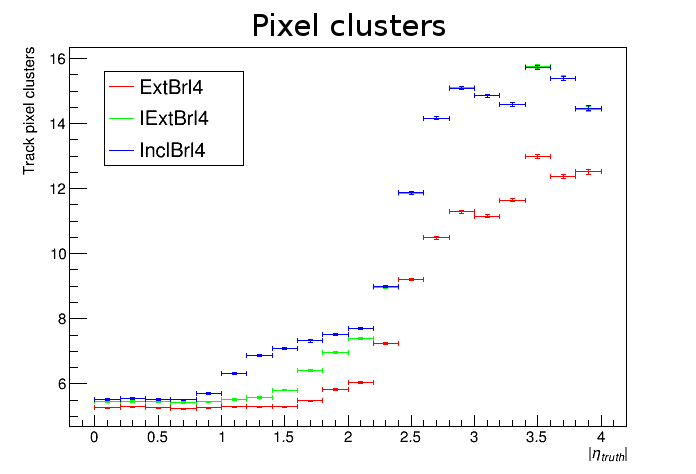
\includegraphics[width=\textwidth]{Tracking/nPixHits_abseta2}
\end{column}
\begin{column}{0.41\textwidth}
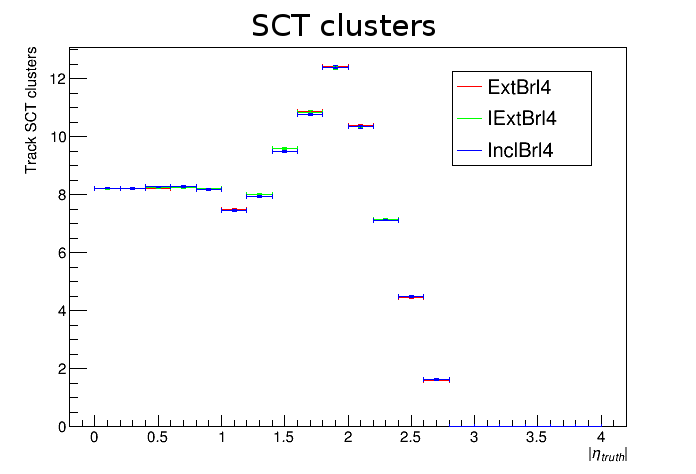
\includegraphics[width=\textwidth]{Tracking/nSCTHits_abseta2}
\end{column}
\begin{column}{0.09\textwidth}
\end{column}
\end{columns}
\vskip-0.1cm

\begin{columns}
\begin{column}{0.09\textwidth}
\end{column}
\begin{column}{0.41\textwidth}
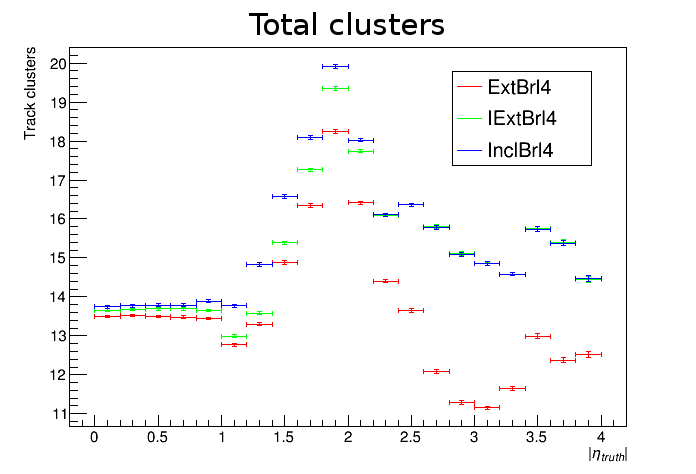
\includegraphics[width=\textwidth]{Tracking/nSiHits_abseta2}
\end{column}
\begin{column}{0.41\textwidth}
\begin{itemize}
\item \small \mbox{ExtBrl4 usa meno cluster.} \\
Diverso approccio nella ricostruzione nella regione ad alto $\eta$
\end{itemize}
\end{column}
\begin{column}{0.09\textwidth}
\end{column}
\end{columns}

\end{frame}

%-----------------------------------------

\begin{frame}
\frametitle{Ricostruzione dei parametri di traccia}
\begin{itemize}
\item[\color{black}--] Parametri di traccia: \textbf{\color{dred}q/\boldmath$p_{T}$}, {\color{dred}\boldmath$\eta$}, {\color{dred}\boldmath$\phi$} (angolo azimuthale), {\color{dred}\boldmath$d_{0}$}
(parametro di impatto trasversale), {\color{dred}\boldmath$z_{0}$} (parametro di impatto longitudinale)
\item[\color{black}--] Per ogni parametro, fit gaussiano della distribuzione di $x_{traccia} - x_{truth}$ in diversi intervalli di $\eta$
	\begin{itemize}
	\item \textbf{Risoluzione:} $\sigma$ estratta dal fit
	%\item \textbf{Bias:} media estratta dal fit
	\end{itemize}
\end{itemize}

\begin{columns}
\begin{column}{.5\textwidth}
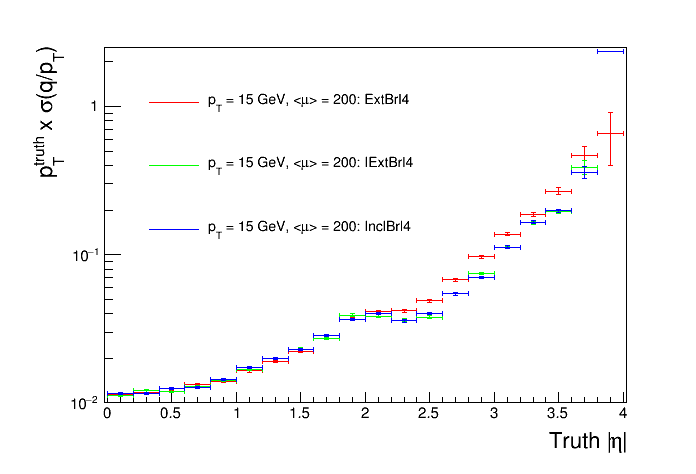
\includegraphics[width=\textwidth]{Tracking/Mixed/pi15pu200_sigQPt_abseta}
\end{column}
\begin{column}{.5\textwidth}
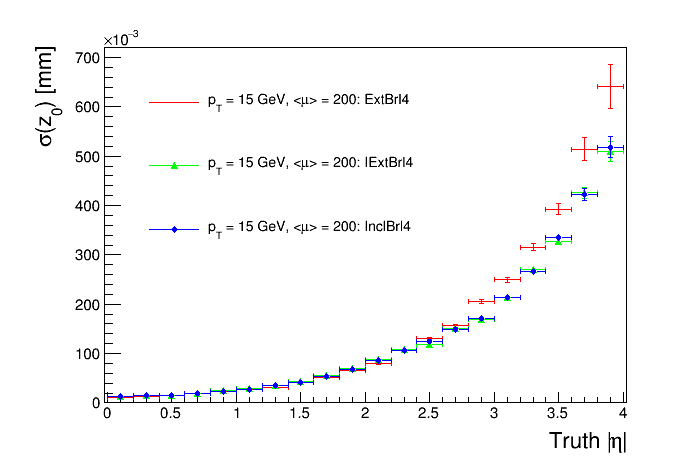
\includegraphics[width=\textwidth]{Tracking/Mixed/pi15pu200_sigZ0_abseta}
\end{column}
\end{columns}
\end{frame}

%-----------------------------------------
\begin{frame}
\frametitle{Tracce mal ricostruite}
Definizione operativa basata sulla distribuzione di $\Delta R_{ricostruito - generato}$:
\centering
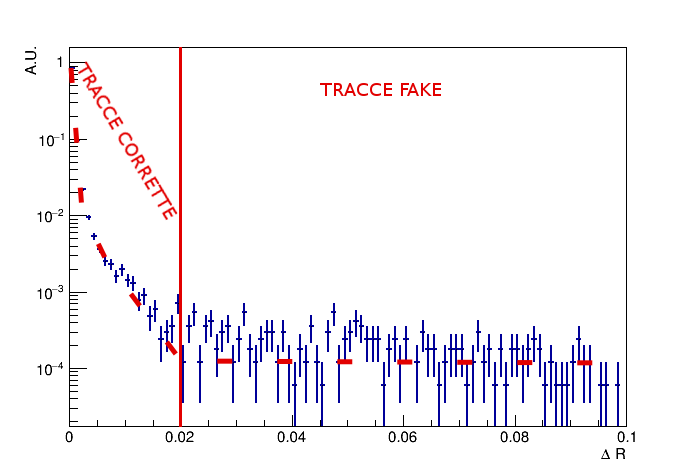
\includegraphics[width=.7\textwidth]{Tracking/pionMatchingDR2}

\begin{itemize}
\item [\color{black}--] Valore ``critico'' di $\Delta R$ dipende dal $p_{T}$
\item[\color{black}--] \textbf{Frazione di tracce mal ricostruite = } (0.5 $\div$ 4) \%
\end{itemize}
\end{frame}

%-----------------------------------------

\begin{frame}[t]
\frametitle{Efficienza di ricostruzione}
\begin{block}{\color{dred}Definizione}
$\epsilon\ (\eta \in\ $bin$_{i}) = $ P(traccia correttamente ricostruita $\vert$ $\eta_{generato} \in$ bin$_{i}$)
\end{block}
\bigskip

\begin{columns}
\begin{column}{.5\textwidth}
\centering
\ \ \ \ $\langle\mu\rangle$ = 200, confronto layout
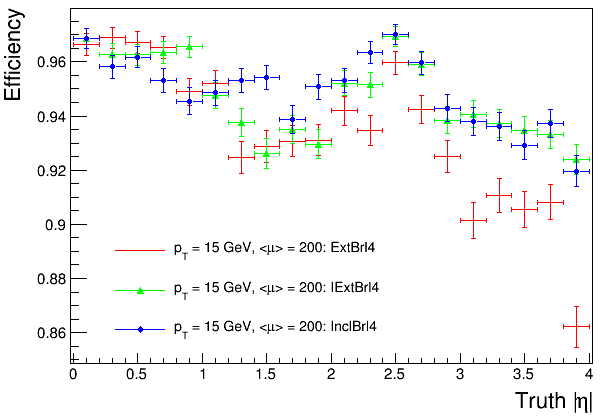
\includegraphics[width=\textwidth]{Tracking/Mixed/pi15pu200_eff_abseta}
\end{column}
\begin{column}{.5\textwidth}
\centering
\ \ \ \ Fully Inclined layout, confronto pile-up
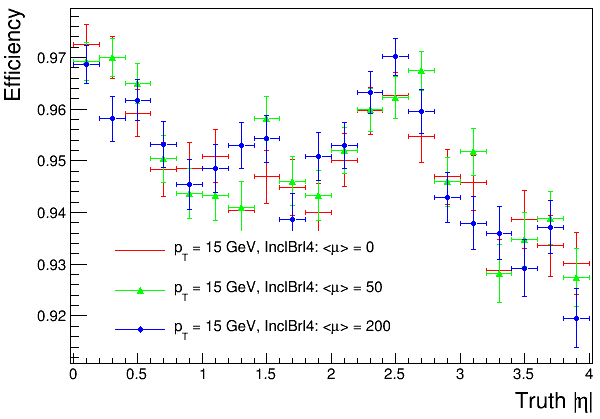
\includegraphics[width=\textwidth]{Tracking/InclBrl4/pi15_eff_abseta}
\end{column}
\end{columns}
\medskip
Efficienza media dipendente dal $p_{T}$: (90 $\div$ 95)\ \%
\end{frame}

%-----------------------------------------
\begin{frame}
\frametitle{Studio di singola particella - sommario}
Abbiamo valutato le prestazioni del tracciatore in campioni di singola
particella e condizioni di pile-up realistiche:
\begin{itemize}
\item Non \`e stata osservato un apprezzabile peggioramento delle prestazioni
all'aumentare del pile-up
\item I layout ''inclined'' si comportano mediamente meglio, ma quello 
''extended'' deve essere ottimizzato
\item Risoluzioni ed efficienze rispettano i requisiti desiderati
\end{itemize}

\end{frame}

\section{}
%-----------------------------------------
\begin{frame}


\Large{\color{gray}1. Studio di singola particella}\\
\bigskip
\bigskip
\bigskip
\Large{\color{dred}2. Studio del canale $H \rightarrow ZZ^{*} \rightarrow 4\mu$}

\end{frame}


\section{Studio del bosone di Higgs in 4 muoni}
%-----------------------------------------

\begin{frame}[t]
\frametitle{Motivazioni dello studio}

\textbf{\color{dred}Obiettivo}
\begin{itemize}
\item[\color{black}$\Rightarrow$] \small Verificare adeguatezza dei layout in questo canale
\end{itemize}
\medskip
\textbf{Perch\'e studiare il bosone di Higgs?}
\begin{itemize}
\item[\color{black}$\Rightarrow$] \small \`E uno degli obiettivi principali di HL-LHC (conferma SM o nuova fisica)
\end{itemize}

\textbf{Perch\'e il canale di decadimento in 4 muoni?}
\begin{itemize}
\item[\color{black}$\Rightarrow$] \small Pur non essendo un canale particolarmente frequente, ha una segnatura molto pulita
\end{itemize}

\textbf{Perch\'e il canale di produzione gluon-gluon fusion?}
\begin{itemize}
\item[\color{black}$\Rightarrow$] \small \`E il canale di produzione pi\`u frequente ad LHC, e d\`a luogo ad un singolo
Higgs senza jet associati $\rightarrow$ pi\`u semplice per la tracciatura
\end{itemize}

\begin{columns}
\begin{column}{.5\textwidth}
\centering
%Produzione
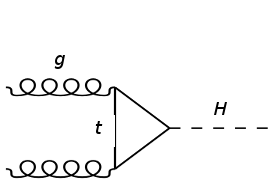
\includegraphics[width=.5\textwidth,height=2.5cm]{ggF2}
\end{column}
\begin{column}{.5\textwidth}
\centering
%Decadimento
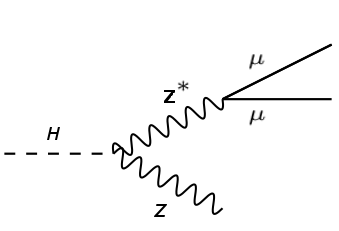
\includegraphics[width=.5\textwidth,height=2.5cm]{HZZ4mu_12}
\end{column}
\end{columns}

\end{frame}
%-----------------------------------------

\begin{frame}[t]
\frametitle{Metodo di simulazione veloce}
\centering
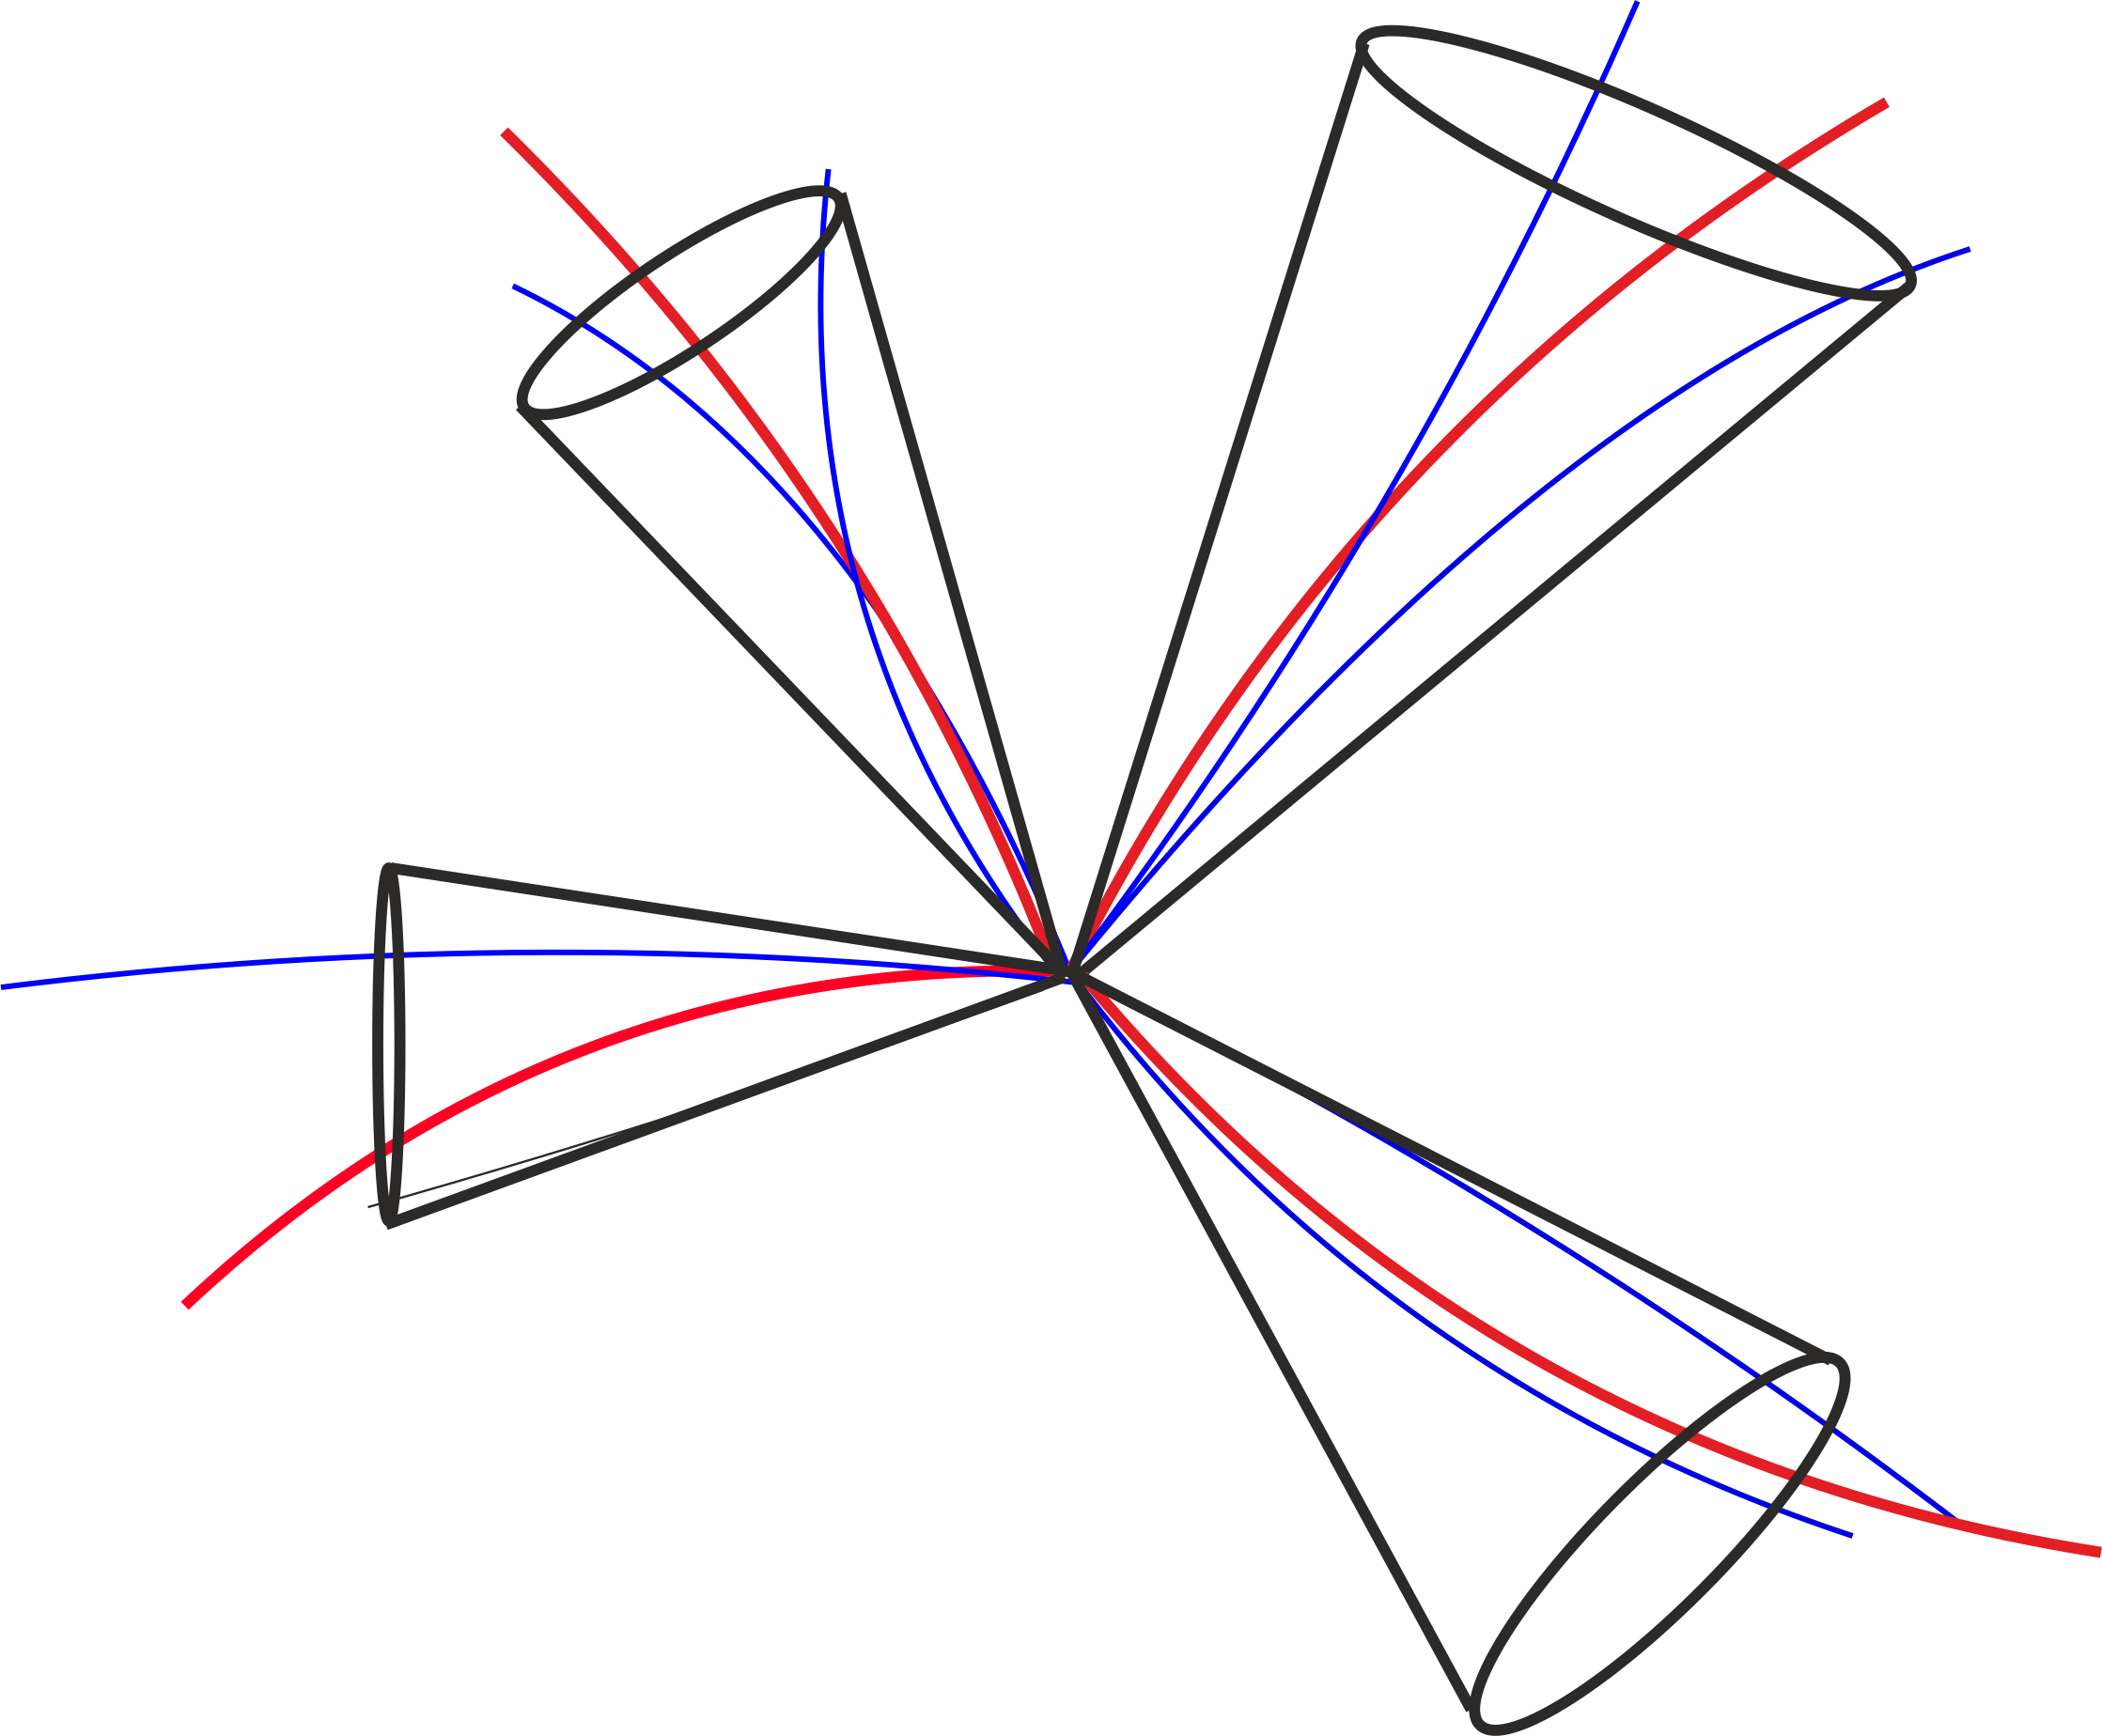
\includegraphics[width=.6\textwidth, height=6cm]{cone_3}

\begin{itemize}
\item Regione di interesse (RoI) definita per ogni muone in $H \rightarrow 4\mu$
\item Stesso campione generato di $H \rightarrow 4\mu$ per i confronti tra layout
\end{itemize}

\end{frame}

%-----------------------------------------
\begin{comment}
\begin{frame}[t]
\frametitle{Generazione dell'evento}
\vskip-0.4cm
\begin{block}{}
\begin{itemize}
\item 50'000 eventi di $gg\rightarrow H \rightarrow ZZ^{*} \rightarrow 4\mu$ (segnale) \tikzmark{topbrace}
\item 16'000 eventi di $ZZ^{(*)} \rightarrow 4\mu$ (fondo) \tikzmark{bottombrace}
\end{itemize}
\begin{tikzpicture}[overlay, remember picture]
\draw [decoration={brace,amplitude=0.5em},decorate,ultra thick,black]
let \p1=(topbrace), \p2=(bottombrace) in
({max(\x1,\x2)}, {\y1+0.8em}) -- node[right=0.6em] {POWHEG} ({max(\x1,\x2)}, {\y2});
\end{tikzpicture}
\setbeamercolor{local structure}{fg=dred} 
\vskip-.5cm
\begin{itemize}
\item $\langle\mu\rangle$ = 200 (Pythia8), 13 TeV, ExtBrl4, IExtBrl4, InclBrl4 layouts
\item Eventi contenenti 4 muoni + fotoni di final-state-radiation con $p_{T, max}^{\gamma} < 1.5$ GeV
\end{itemize}
%[\color{red}\scalebox{0.9}{\ball}]
%
\end{block}

\begin{columns}
\begin{column}{.5\textwidth}
\centering
%Produzione
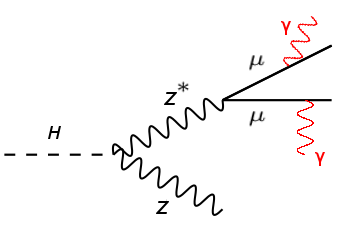
\includegraphics[width=.9\textwidth,height=4cm]{HZZ4mu_22}
\end{column}
\begin{column}{.5\textwidth}
\centering
%Decadimento
$p_{T}$ dei fotoni
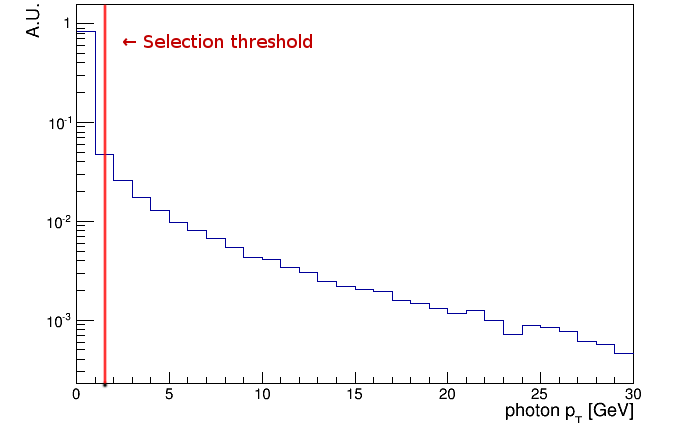
\includegraphics[width=\textwidth, height=4cm]{HZZ4mu/photonPt4}
\end{column}
\end{columns}
\end{frame}
\end{comment}

%-----------------------------------------
\begin{frame}[t]
\frametitle{Generazione dell'evento}
\vskip-0.4cm
\begin{block}{}
\begin{itemize}
\item $gg\rightarrow H \rightarrow ZZ^{*} \rightarrow 4\mu$ (segnale) \tikzmark{topbrace}
\item $ZZ^{(*)} \rightarrow 4\mu$ (fondo) \tikzmark{bottombrace}
\end{itemize}
\begin{tikzpicture}[overlay, remember picture]
\draw [decoration={brace,amplitude=0.5em},decorate,ultra thick,black]
let \p1=(topbrace), \p2=(bottombrace) in
({max(\x1,\x2)}, {\y1+0.8em}) -- node[right=0.6em] {POWHEG} ({max(\x1,\x2)}, {\y2});
\end{tikzpicture}
\setbeamercolor{local structure}{fg=dred} 
\vskip-.5cm
\begin{itemize}
\item $\langle\mu\rangle$ = 200
\item Eventi contenenti 4 muoni + fotoni di final-state-radiation con $p_{T, max}^{\gamma} < 1.5$ GeV
\end{itemize}
%[\color{red}\scalebox{0.9}{\ball}]
%
\end{block}

\begin{columns}
\begin{column}{.5\textwidth}
\centering
%Produzione
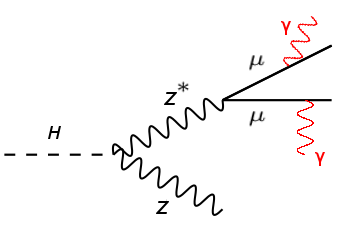
\includegraphics[width=.9\textwidth,height=4cm]{HZZ4mu_22}
\end{column}
\begin{column}{.5\textwidth}
\centering
%Decadimento
$p_{T}$ dei fotoni
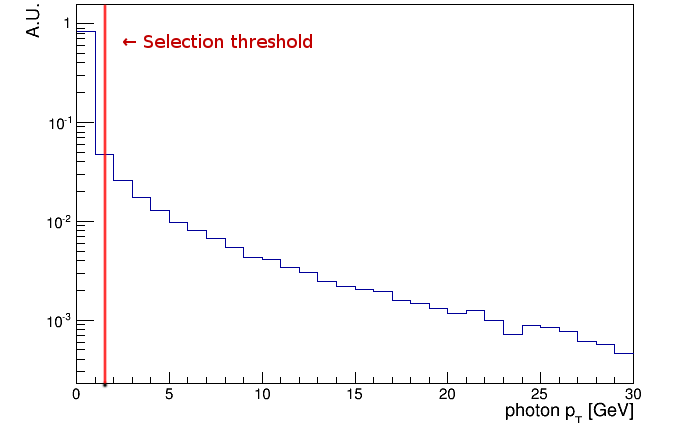
\includegraphics[width=\textwidth, height=4cm]{HZZ4mu/photonPt4}
\end{column}
\end{columns}
\end{frame}

%-----------------------------------------



\begin{frame}
\frametitle{Caratteristiche dei muoni ricostruiti}

\begin{columns}
\begin{column}{.09\textwidth}
\end{column}
\begin{column}{.41\textwidth}
\centering
\onslide<1->{
$p_{T}$
\includegraphics<1->[width=\textwidth]{muonPt2}}
\end{column}
\begin{column}{.41\textwidth}
\centering
\onslide<2->{Muoni con $|\eta| > 4.0$
\includegraphics<2>[width=\textwidth]{truthOutsideDetector2}
\includegraphics<3->[width=\textwidth]{truthOutsideDetector3}}
\end{column}
\begin{column}{.09\textwidth}
\end{column}
\end{columns}

\begin{columns}
\begin{column}{.09\textwidth}
\end{column}
\begin{column}{.41\textwidth}
\centering
\onslide<4->{$p_{T} \times \sigma(q/p_{T})$
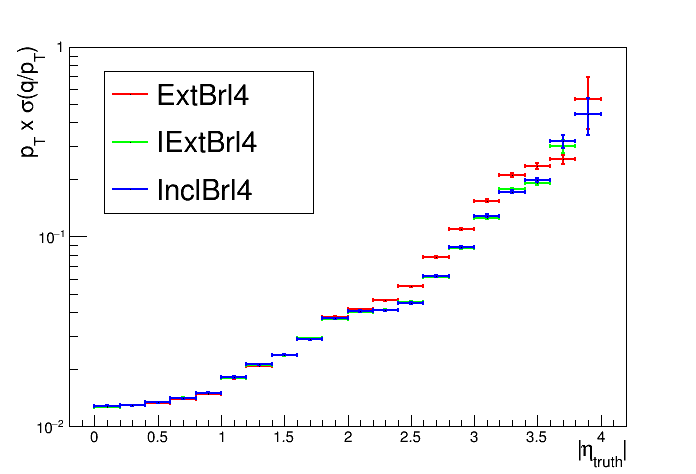
\includegraphics[width=\textwidth]{HZZ4mu/sigQPt_abseta}}
\end{column}
\begin{column}{.41\textwidth}
\centering
\onslide<5->{
Efficienza di ricostruzione
\includegraphics<5->[width=\textwidth]{HZZ4mu/eff_abseta}}
\end{column}
\begin{column}{.09\textwidth}
\end{column}
\end{columns}


\end{frame}
%-----------------------------------------

\begin{frame}
\frametitle{Risoluzione in massa (InclBrl4)}
\setbeamercolor{local structure}{fg=black}
\begin{itemize}
\item[\color{black}--] \small Si ipotizza 100\% di efficienza di identificazione dei muoni per semplicit\`a
\item[\color{black}--] \small Selezione per identificare il segnale e minimizzare il fondo
\end{itemize}

\begin{columns}
\begin{column}{0.09\textwidth}
\end{column}
\begin{column}{0.41\textwidth}
\includegraphics<1>[width=\textwidth]{HZZ4mu/sigRecoOnShellMass_3}
\includegraphics<2>[width=\textwidth]{HZZ4mu/sigRecoOnShellMass_2}
\includegraphics<3>[width=\textwidth]{HZZ4mu/sigRecoOnShellMass}
\end{column}
\begin{column}{0.41\textwidth}
\includegraphics<1>[width=\textwidth]{HZZ4mu/sigRecoOffShellMass_3}
\includegraphics<2>[width=\textwidth]{HZZ4mu/sigRecoOffShellMass_2}
\includegraphics<3>[width=\textwidth]{HZZ4mu/sigRecoOffShellMass}
\end{column}
\begin{column}{0.09\textwidth}
\end{column}
\end{columns}
%\vskip-0.07cm

\begin{columns}
\begin{column}{0.09\textwidth}
\end{column}
\begin{column}{0.41\textwidth}
\includegraphics<1>[width=\textwidth]{HZZ4mu/sigRecoMass_3}
\includegraphics<2>[width=\textwidth]{HZZ4mu/sigRecoMass_2}
\includegraphics<3>[width=\textwidth]{HZZ4mu/sigRecoMass}
\end{column}
\begin{column}{0.41\textwidth}
\begin{itemize}
\item \small All'aumentare di $\eta$, la risoluzione peggiora a causa della perdita
di risoluzione in $p_{T}$ delle tracce
\end{itemize}
\end{column}
\begin{column}{0.09\textwidth}
\end{column}
\end{columns}

\end{frame}

%-----------------------------------------
\begin{frame}[t]
\frametitle{Significativit\`a del canale}
\begin{center}
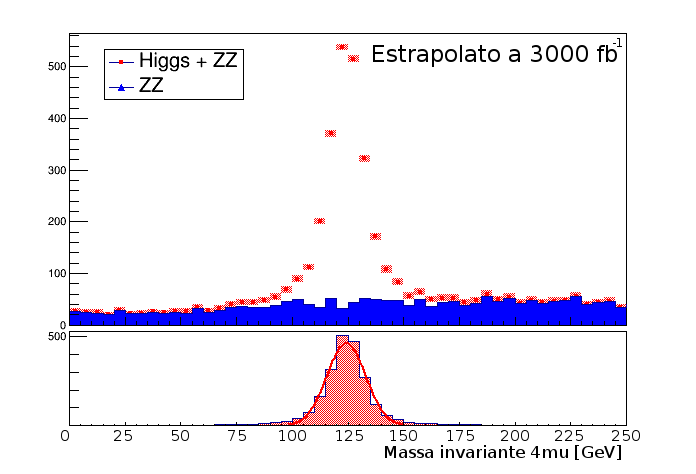
\includegraphics[width=.5\textwidth]{SBInclBrl4_2}
\end{center}

\begin{itemize}
\item \small Segnale e fondo definiti come il numero di eventi in una regione ampia
\mbox{$\pm$ 1.5 $\times \sigma_{H}$} attorno al picco
\item \small Significativit\`a = $\frac{S}{\sqrt{S + B}}$
\item \small $\mu$ = $\frac{(\sigma \times BR)_{mis.}}{(\sigma \times BR)_{SM}}$ $\rightarrow 
\Delta\mu/\mu \simeq \frac{\sqrt{S + B}}{S}$ (stat.)
\end{itemize}
\end{frame}

%----------------------------------------------

\begin{frame}
\frametitle{Significativit\`a del canale - Risultati}
\centering
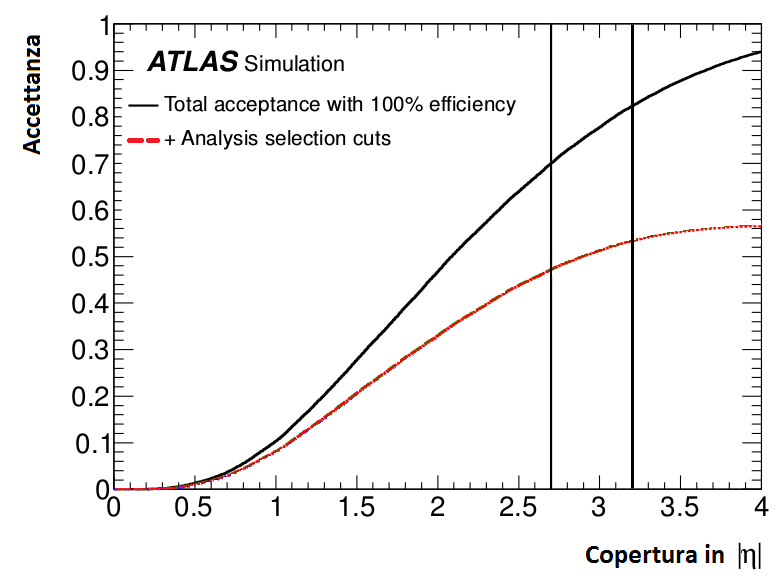
\includegraphics[width=.5\textwidth]{scopingAcceptance2}\\
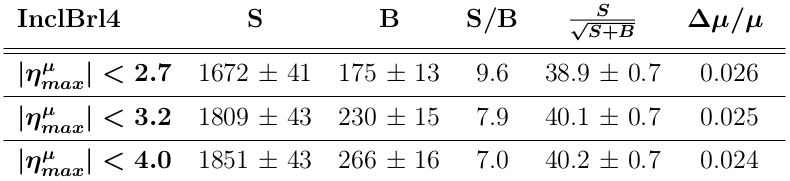
\includegraphics[width=.9\textwidth]{significanceInclBrl4}\\
\begin{flushleft}
\framebox{\small S, B: numero di eventi estrapolati a 3000 fb$^{-1}$}
\end{flushleft}
\end{frame}


\section{}
%-----------------------------------------
\begin{frame}
\frametitle{Conclusioni - 1}
\begin{itemize}
\item<1-> Abbiamo sviluppato e applicato una tecnica di simulazione veloce
su campioni di fisica, testandone l'efficacia sullo studio delle prestazioni di ITk;
\item<2-> I layout proposti dalla collaborazione sono robusti rispetto al pile-up;
\item<3-> Abbiamo misurato il canale $H \rightarrow ZZ^{*} \rightarrow 4\mu$ con
un rapporto segnale/fondo di almeno 7 in tutte le regioni angolari e con un'incertezza
su $\mu$ del 2.5\% (senza includere altre incertezze sistematiche);
\item<4-> In generale, i layout ``inclined'' mostrano prestazioni migliori rispetto a quello
``extended'', ma quest'ultimo soffre della mancanza di un algoritmo di ricostruzione ottimizzato.
\end{itemize}
\end{frame}

%-----------------------------------------
\begin{frame}[label=Conclusions]
\frametitle{Conclusioni - 2}
\onslide<1->{
Quindi:\\
\setbeamercolor{local structure}{fg=dred} 
\begin{itemize}
\item<2-> A questo stadio preliminare \`e presto per trarre conclusioni sulla scelta del layout,
ma questi studi sono utili per mostrare che tutti i progetti rispettano approssimativamente 
i requisiti necessari;
\item<3-> L'estensione della copertura angolare a 3.2 fornisce un buon aumento della statistica, mentre estendere ulteriormente a 4.0 non \`e particolarmente utile, limitatamente
al canale fisico studiato.

\end{itemize}}

\bigskip
\bigskip
\bigskip
\onslide<4-> {
\centering
\Large \color{dred} Grazie per l'attenzione
}

\end{frame}

%-----------------------------------------
\begin{frame}
\begin{center}
\huge{\color{dred}Backup slides}
\end{center}
\end{frame}
%-----------------------------------------
%-----------------------------------------
%-----------------------------------------
%-----------------------------------------
%-----------------------------------------
%-----------------------------------------
%-----------------------------------------
\begin{frame}
\frametitle{Inner Detector}
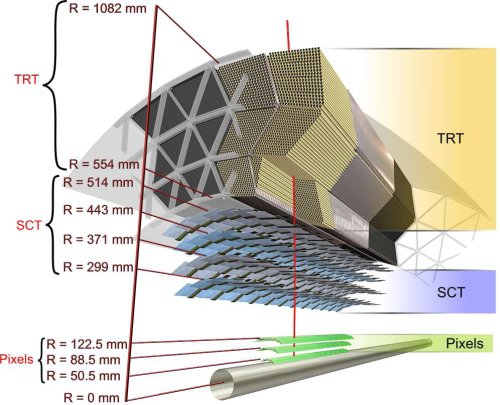
\includegraphics[width=\textwidth]{innerdetector_sideways}
\end{frame}

\begin{frame}
\frametitle{Pixel - Run 1}
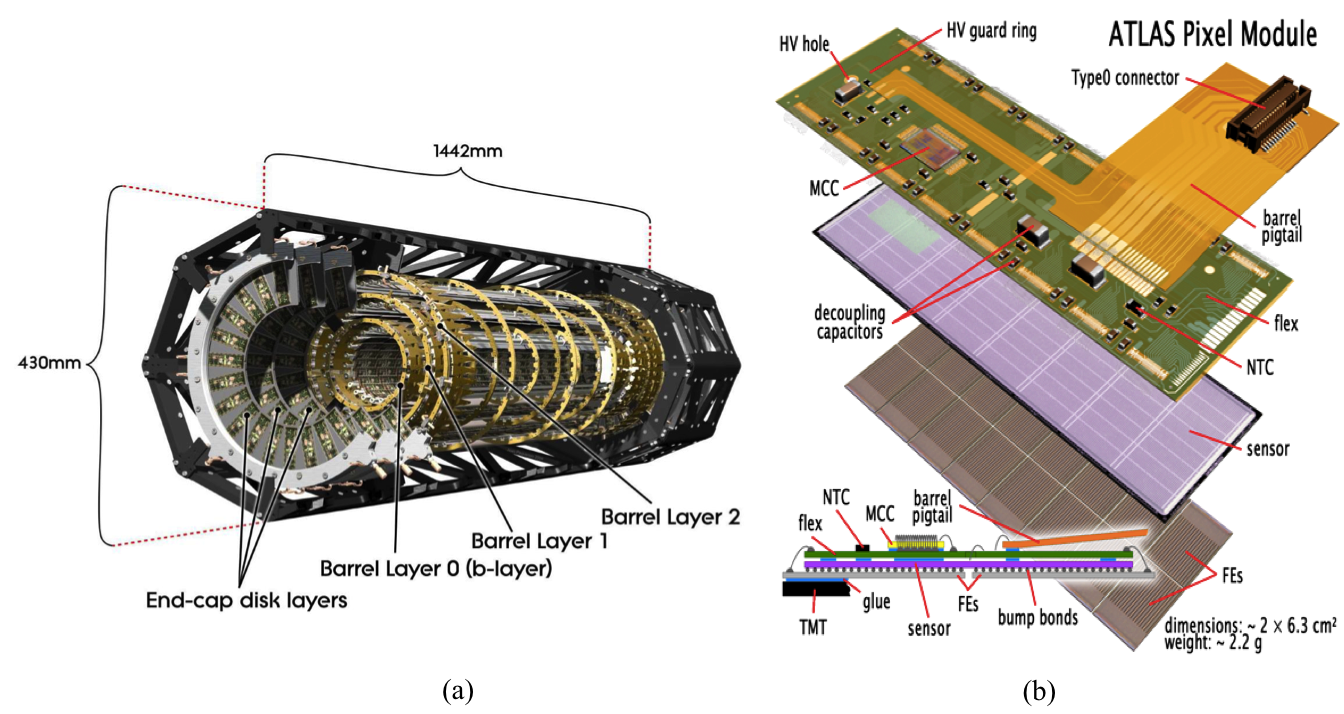
\includegraphics[width=\textwidth]{Pixel_run1}
\end{frame}

\begin{frame}
\frametitle{Formazione di ``long cluster''}
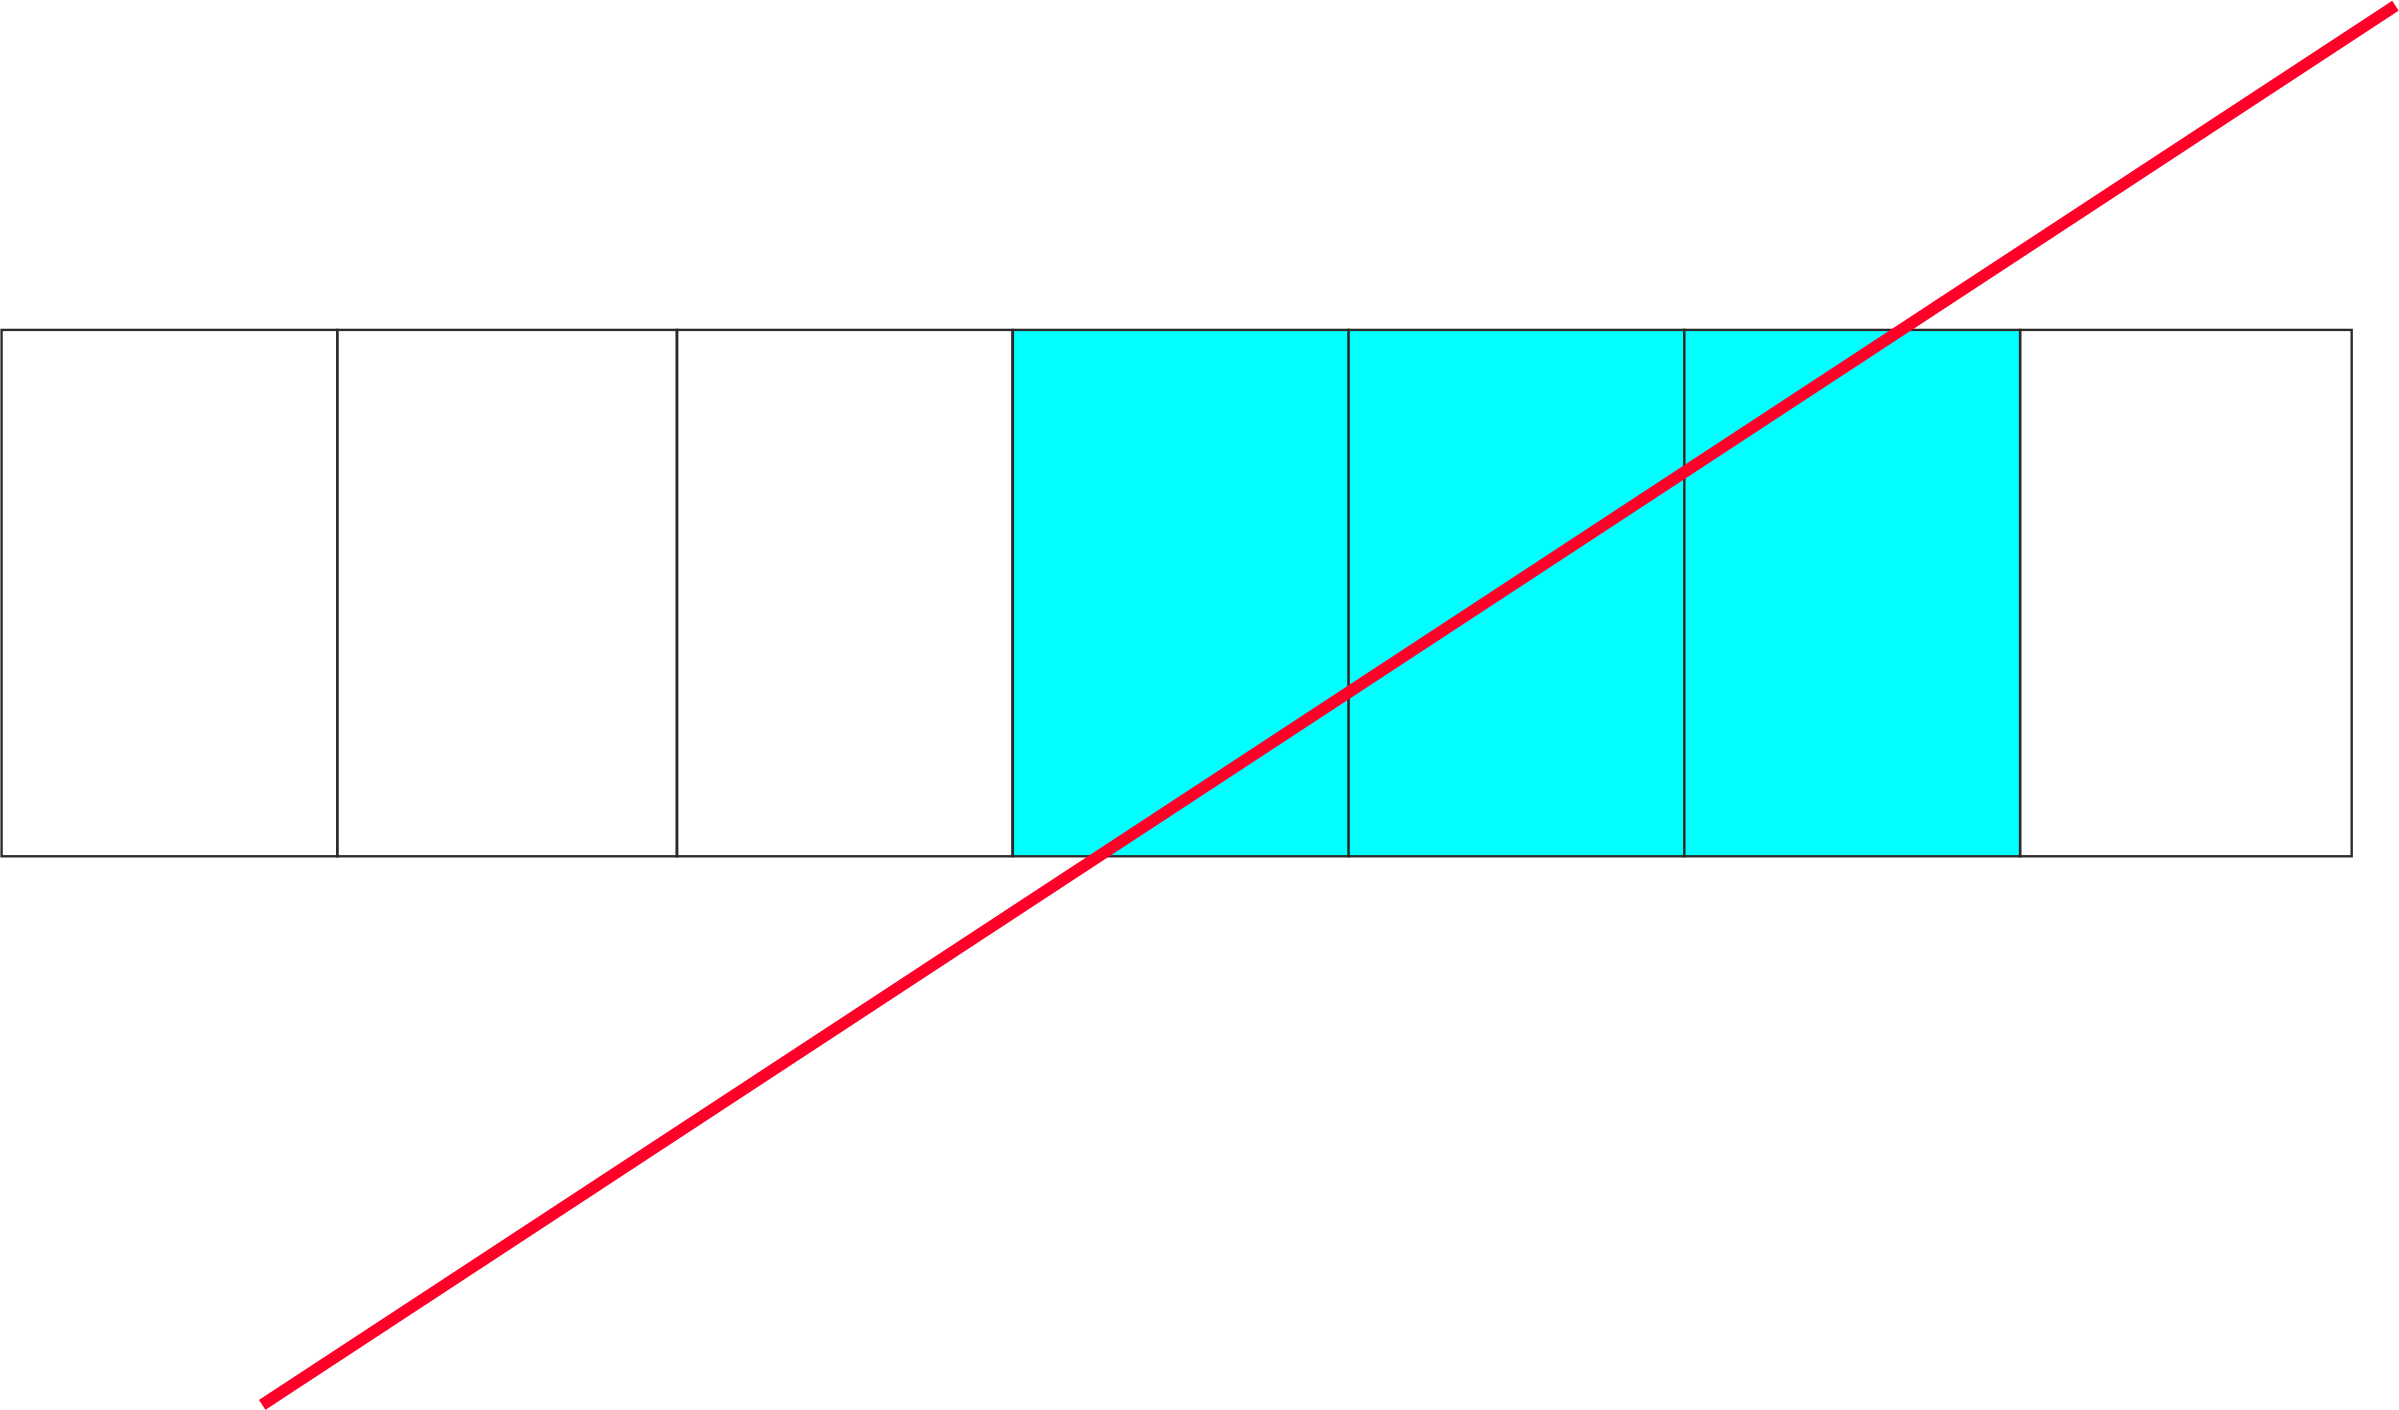
\includegraphics[width=\textwidth]{long_cluster}
\end{frame}

\begin{frame}
\frametitle{Materiale}
\begin{columns}
\begin{column}{.5\textwidth}
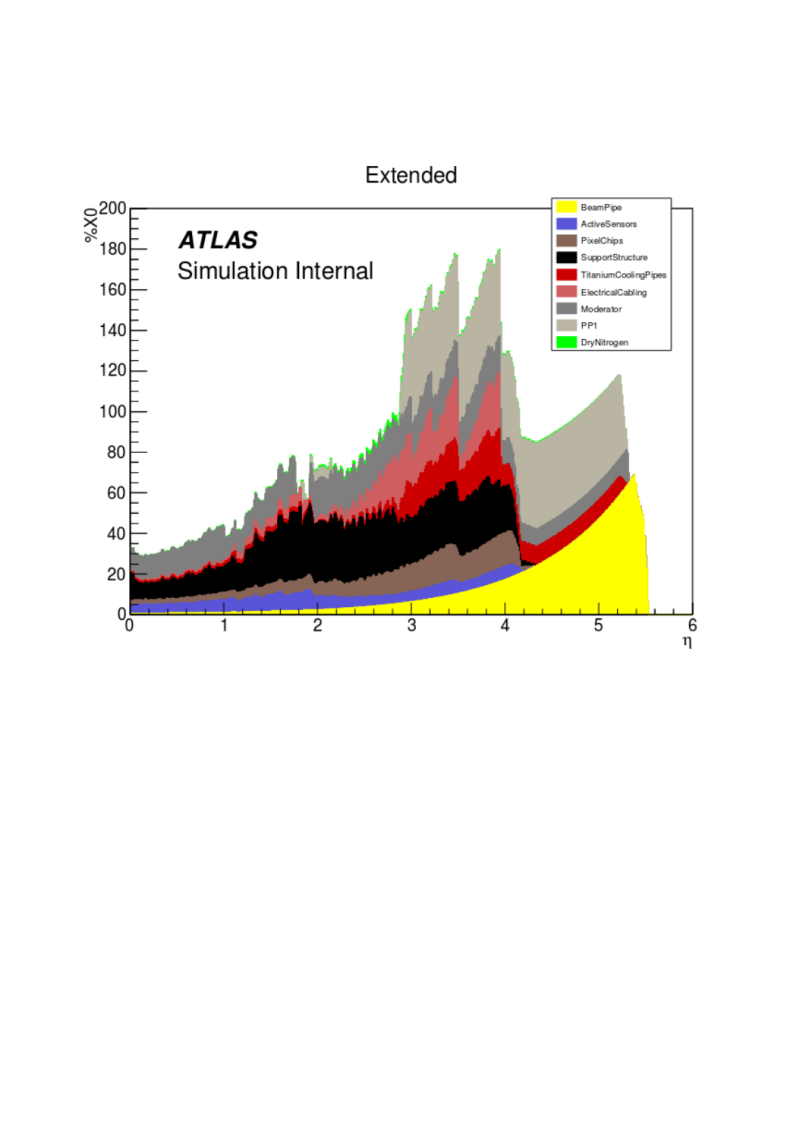
\includegraphics[width=\textwidth]{Ext_material}
\end{column}
\begin{column}{.5\textwidth}
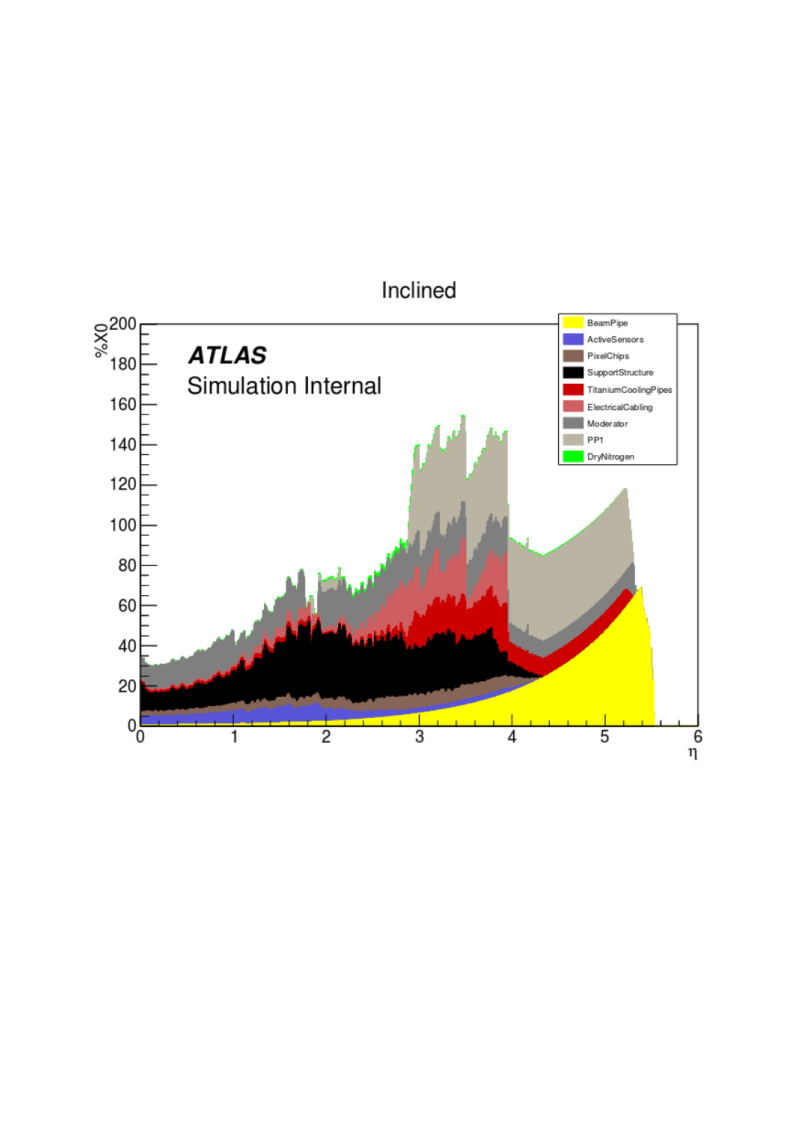
\includegraphics[width=\textwidth]{Incl_material}
\end{column}
\end{columns}
\end{frame}

\begin{frame}
\frametitle{Occupancy}
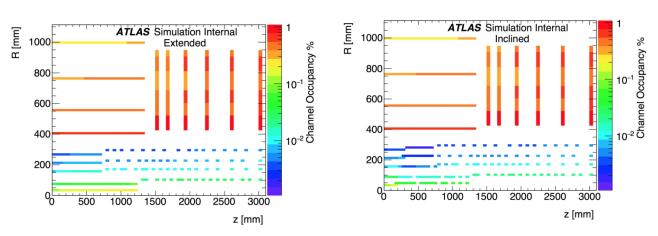
\includegraphics[width=\textwidth]{occupancy}
\end{frame}

\begin{frame}[t]
\frametitle{Stabilit\`a con $\Delta$R}
\begin{columns}
\begin{column}{.5\textwidth}
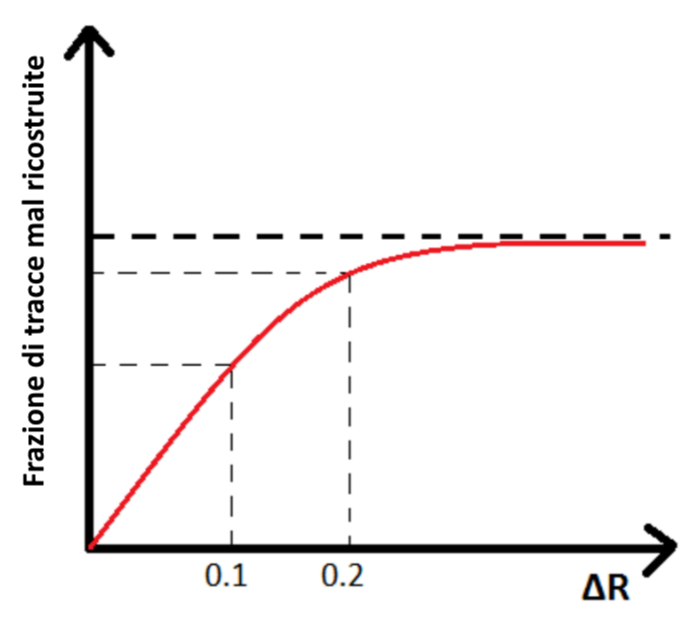
\includegraphics[width=\textwidth]{fakeProbVsDR}
\end{column}
\begin{column}{.5\textwidth}
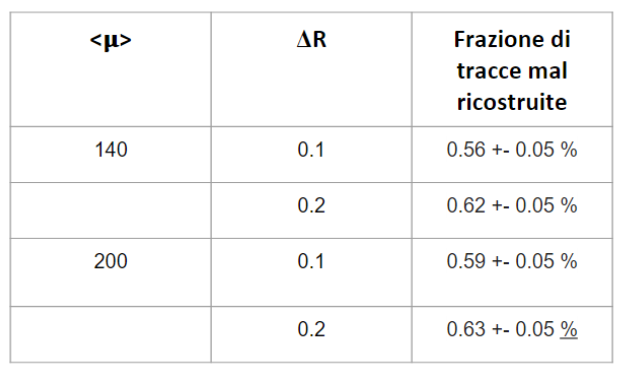
\includegraphics[width=\textwidth, height=4cm]{fakeProbVsDR_tab}
\end{column}
\end{columns}
\bigskip
\bigskip
\bigskip
Leggero aumento in funzione dell'ampiezza della regione di interesse
\end{frame}


\begin{frame}
\frametitle{Tracce generate e ricostruite}
\begin{columns}
\begin{column}{.09\textwidth}
\end{column}
\begin{column}{.41\textwidth}
\centering
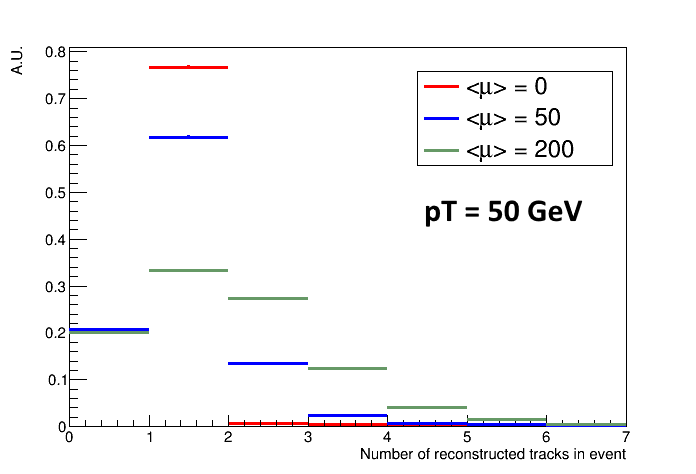
\includegraphics[width=\textwidth]{Tracking/nRecoTracks}
\end{column}
\begin{column}{.41\textwidth}
\centering
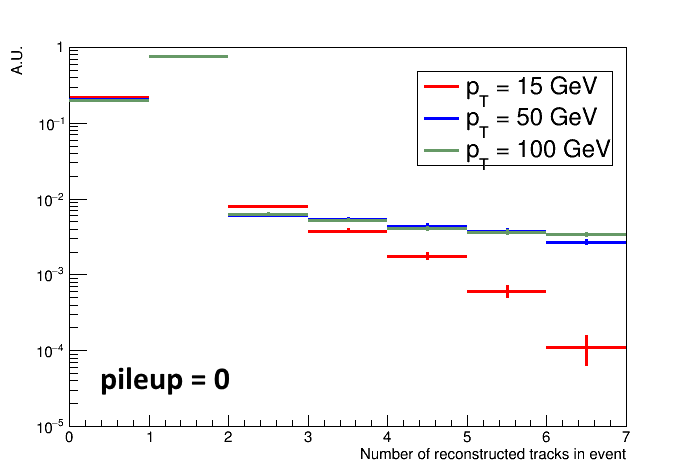
\includegraphics[width=\textwidth]{Tracking/nRecoTracks_pt}
\end{column}
\begin{column}{.09\textwidth}
\end{column}
\end{columns}

\begin{columns}
\begin{column}{.09\textwidth}
\end{column}
\begin{column}{.41\textwidth}
\centering
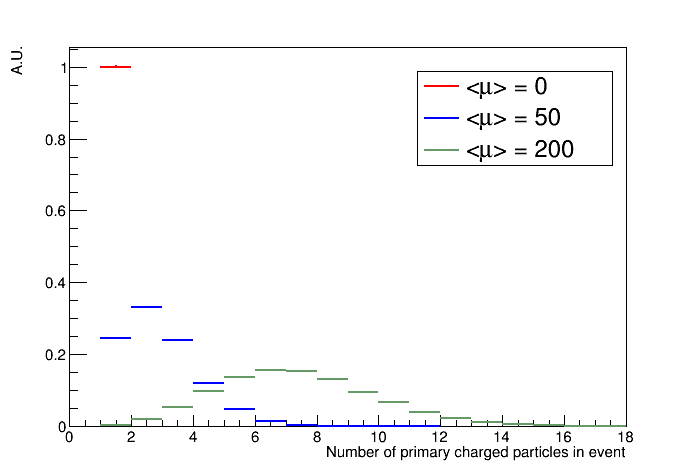
\includegraphics[width=\textwidth]{Tracking/nPrimaryChargedTruth}
\end{column}
\begin{column}{.41\textwidth}
\centering
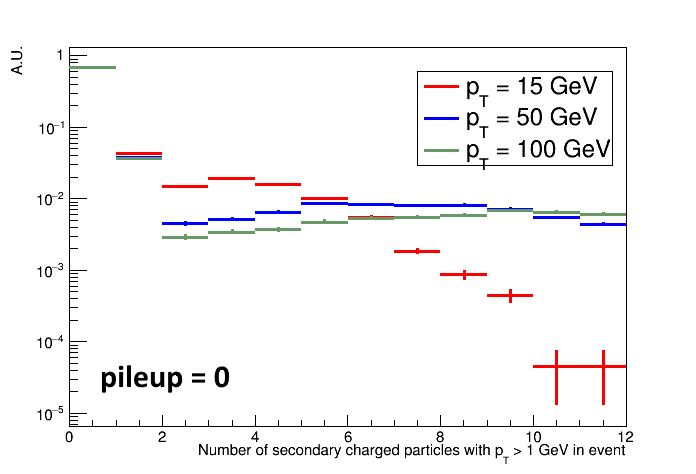
\includegraphics[width=\textwidth]{Tracking/nSecondaryChargedTruth1GeV_pt}
\end{column}
\begin{column}{.09\textwidth}
\end{column}
\end{columns}
\end{frame}


\begin{frame}
\frametitle{Fast vs full simulation}
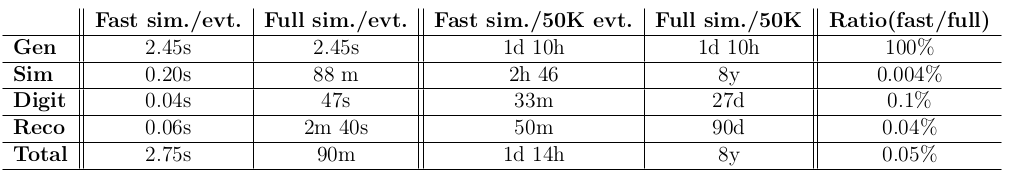
\includegraphics[width=\textwidth]{time}
\end{frame}

\begin{frame}[t]
\frametitle{Selezione dell'analisi}

La selezione viene applicata sequenzialmente:
\begin{itemize}
\item<1-> l'evento deve contenere almeno 4 tracce;
\item<2-> ogni traccia deve essere formata da almeno 10 cluster;
\item<3-> ogni traccia deve avere $p_{T} >$ 6 GeV;
\item<4-> la distanza tra lo $z_{0}$ della traccia e il vertice primario (truth) deve essere $< 5\sigma_{z}$;
\end{itemize}
\medskip
\pause
\pause
\pause
\pause
\`E stato verificato che a questo punto tutti gli eventi hanno non pi\`u di 4 tracce $\rightarrow$ tagli topologici:
\begin{itemize}
\item<6-> le tracce devono essere isolate: $\sum_{\Delta R < 0.1} (p_{T}) / p_{T, candidate} <$ 1;
\item<7-> ci devono essere due paia di tracce con carica opposta;
\item<8-> Il $p_{T}$ ordinato delle tracce deve essere ($>$ 20, $>$ 15, $>$10, $>$ 6) GeV;
\item<9-> almeno uno dei candidati off-shell
deve avere $|\eta| <$ 2.7;
\item<10-> la massa del paio on-shell deve stare nell'intervallo [50,106] GeV;
\item<11-> la massa del paio off-shell deve stare nell'intervallo [12,115] GeV;
\end{itemize}

\end{frame}

%----------------------------------------------

\begin{frame}[t]
\frametitle{Distribuzione di massa dei bosoni Z}

\begin{itemize}
\item[\color{black}--] On-shell: Z con massa pi\`u vicina a quella di riposo
\end{itemize}
\bigskip
\begin{columns}
\begin{column}{.5\textwidth}
\centering
$H \rightarrow ZZ^* \rightarrow 4\mu$
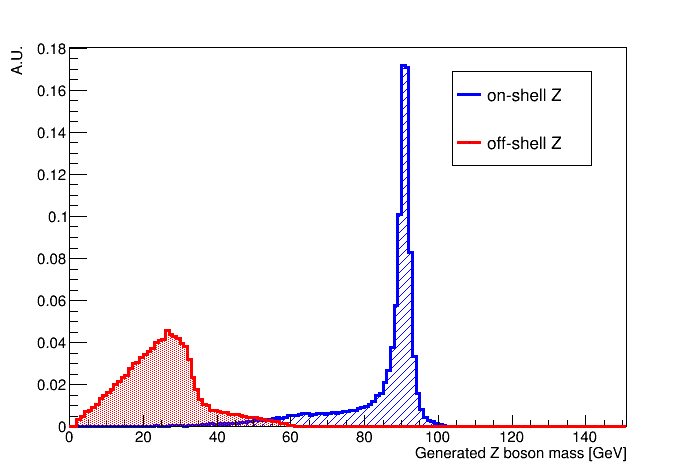
\includegraphics[width=\textwidth]{HZZ4mu/genZMass}
\end{column}
\begin{column}{.5\textwidth}
\centering
$ZZ^{(*)} \rightarrow 4\mu$\par
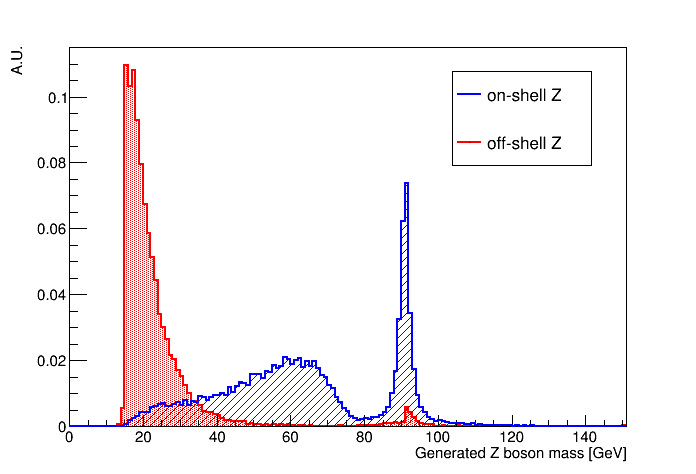
\includegraphics[width=\textwidth]{ZZ4mu/genZMass}
\end{column}
\end{columns}

\begin{columns}
\begin{column}{.6\textwidth}
\end{column}
\begin{column}{.4\textwidth}
Picco {\color{dred} off-shell} a $\sim$ 90 GeV: componente ZZ del fondo
\end{column}
\end{columns}

\end{frame}

%-----------------------------------------


%-----------------------------------------
\begin{frame}
\frametitle{Significativit\`a e incertezze }

Definizione significativit\`a:\\
\begin{itemize}
\item[\color{black}-] Dati distanti n$\sigma$ dal fondo
	\begin{itemize}
	\item $(S + B) - n\sqrt{S + B} > B \rightarrow \frac{S}{\sqrt{S+B}} > n$
	\end{itemize}		
\end{itemize}

\bigskip
\bigskip

Incertezza sul parametro $\mu$:
\begin{itemize}
\item $\mu = \frac{(\sigma \times BR)_{meas}}{\sigma \times BR)_{SM}}$
\item $S = \sigma \times BR \times \int\mathcal{L}dt \times \epsilon$
\item $\Delta S_{meas} = \Delta((S + B) - B) = \sqrt{S + B}$
\item $\Delta\mu/\mu = \Delta S_{meas}/ S = \sqrt{S+B}/S$
\end{itemize}

\end{frame}

%-----------------------------------------
\begin{frame}
\frametitle{Truth mass + pt selection}
\begin{columns}
\begin{column}{.5\textwidth}
\centering
Massa invariante di $4\mu$ (fondo)
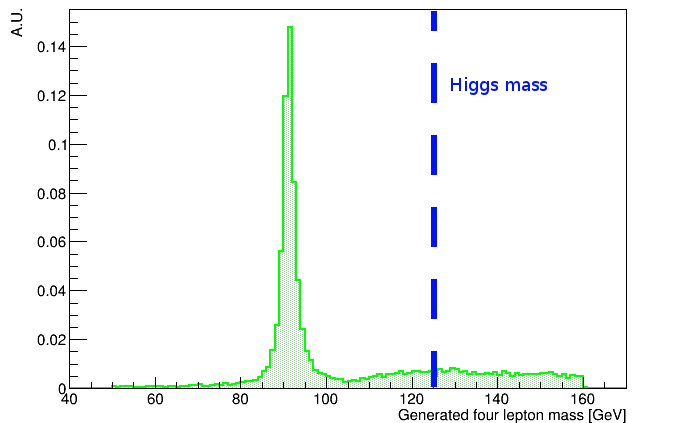
\includegraphics[width=\textwidth]{ZZ4mu/gen4muMass4}
\end{column}
\begin{column}{.5\textwidth}
\centering
$p_{T}$ dei fotoni\par
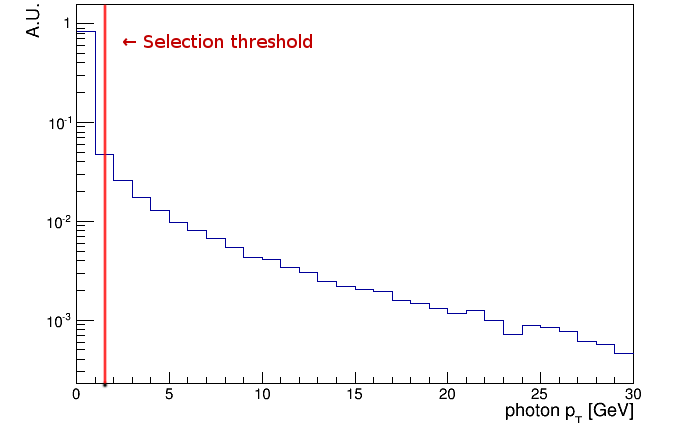
\includegraphics[width=\textwidth]{HZZ4mu/photonPt4}
\end{column}
\end{columns}
\end{frame}
%-----------------------------------------

\begin{frame}[t]
\frametitle{Metodo di simulazione veloce}

\only<1>{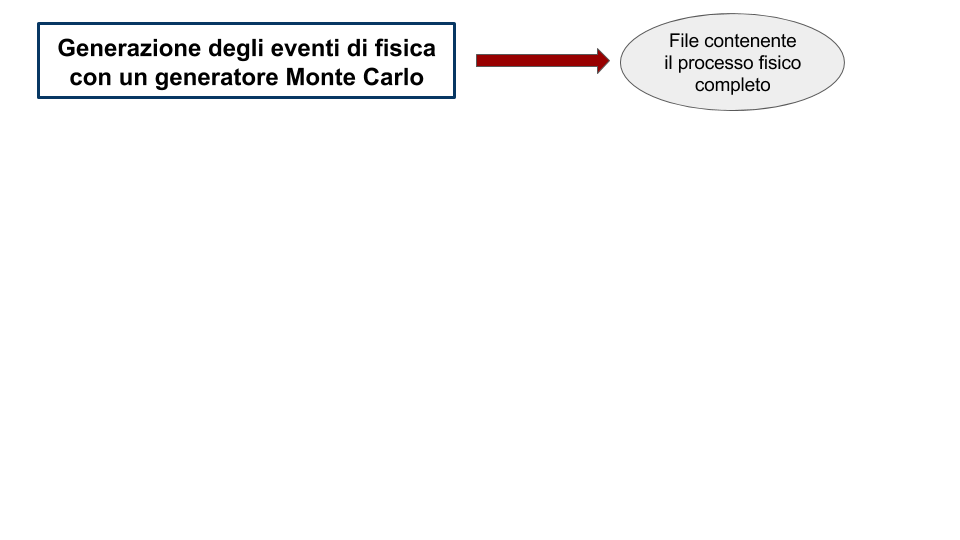
\includegraphics[width=\textwidth]{PhysicsGenerationFlowIT}}
\only<2>{\includegraphics[width=\textwidth]{PhysicsGenerationFlowIT2}}
\only<3>{\includegraphics[width=\textwidth]{PhysicsGenerationFlowIT3}}
\only<4>{\includegraphics[width=\textwidth]{PhysicsGenerationFlowIT4}}

\end{frame}

\end{document}